%% ****** Start of file aiptemplate.tex ****** %
%%
%%   This file is part of the files in the distribution of AIP substyles for REVTeX4.
%%   Version 4.1 of 9 October 2009.
%%
%
% This is a template for producing documents for use with 
% the REVTEX 4.1 document class and the AIP substyles.
% 
% Copy this file to another name and then work on that file.
% That way, you always have this original template file to use.

%\documentclass[aip,graphicx]{revtex4-1}
%\documentclass[aip,reprint]{revtex4-1}

%\usepackage{graphicx}

%\draft % marks overfull lines with a black rule on the right
%\documentclass[pre,aps,floatfix,authordate1-4,twocolumn]{revtex4-1}
%\documentclass[pre,aps,floatfix,authordate1-4]{revtex4-1}

\documentclass[aip,jcp,twocolumn]{revtex4}
%\documentclass[aip,jcp]{revtex4}
%\documentclass{article}



%\documentclass[aps,prl,preprint,groupedaddress]{revtex4}

\usepackage{rotating} 
\usepackage{times}
\usepackage{graphicx}
\usepackage{setspace}
\usepackage{amsmath}
\usepackage{epstopdf}
\usepackage[obeyFinal]{easy-todo}
\usepackage{csquotes}
\usepackage{mhchem}
\usepackage{chemfig}

%\usepackage{markdown} 

\begin{document}

% Use the \preprint command to place your local institutional report number 
% on the title page in preprint mode.
% Multiple \preprint commands are allowed.
%\preprint{}

\title{Accurate binding of calcium to phospholipid bilayers by effective inclusion of electronic polarization} %Title of paper

% repeat the \author .. \affiliation  etc. as needed
% \email, \thanks, \homepage, \altaffiliation all apply to the current author.
% Explanatory text should go in the []'s, 
% actual e-mail address or url should go in the {}'s for \email and \homepage.
% Please use the appropriate macro for the type of information

% \affiliation command applies to all authors since the last \affiliation command. 
% The \affiliation command should follow the other information.

\author{Josef Melcr}
\author{Hector Martinez-Seara Monne}
\affiliation{Institute of Organic Chemistry and Biochemistry,
Academy of Sciences of the Czech Republic, 
Prague 6, Czech Republic}
\author{Pavel Jungwirth}
\affiliation{Institute of Organic Chemistry and Biochemistry,
Academy of Sciences of the Czech Republic, 
Prague 6, Czech Republic}
\affiliation{Department of Physics, Tampere University of Technology, P.O. Box 692, FI-33101
Tampere, Finland}

\author{O. H. Samuli Ollila}
\email[]{samuli.ollila@helsinki.fi}
%\homepage[]{Your web page}
\affiliation{Institute of Organic Chemistry and Biochemistry,
Academy of Sciences of the Czech Republic, 
Prague 6, Czech Republic}
\affiliation{Institute of Biotechnology, University of Helsinki}


% Collaboration name, if desired (requires use of superscriptaddress option in \documentclass). 
% \noaffiliation is required (may also be used with the \author command).
%\collaboration{}
%\noaffiliation

\date{\today}

\begin{abstract}
  % insert abstract here
  Despite of the significant biological relevance, the binding details of cations in cellular
  lipid membranes are not fully understood. For example, consistent results for
  the binding affinities and stoichimetries of Na$^+$ and Ca$^{2+}$ ions to phospholipid bilayers have not been
  achieved with different experimental and theoretical methods. As recently shown in the 
  NMRlipids project, a Open Collaboration running at \url{nmrlipids.blogspot.com},
  the ion binding details could be resolved with unprecendent detail by intepreting
  the experimental NMR data with classical molecular dynamics (MD) simulations.
  However, the accuracy of the existing lipid models for MD simulations was not sufficient for this.
  In this work we show that the binding details of Na$^+$ and Ca$^{2+}$ ions to
  1-Palmitoyl-2-oleoylphosphatidylcholine (POPC) bilayer
  can be accurately described with a MD simulation model having implicitly included electronic polarization.
  This is demonstrated by applying the electronic continuum correction (ECC) to a
  state of the art lipid model for MD simulations of POPC
  lipid bilayer. The introduced ECC-lipid model reproduces the experimentally measured structural parameters for the ion-free membrane,
  the response of lipid headgroup to the bound positive charge, and the binding affinities of
  Na$^+$ and Ca$^{2+}$ ions. The imperceptible binding of Na$^+$ ions to POPC bilayer
  and interactions of Ca$^{2+}$ mainly with phoshpate oxygens in the ECC-lipid model give
  support to the early intepretations of the experimental spectroscopic data.
  On the other hand, Ca$^{2+}$ ions form complexes with 1-3 lipid molecules with almost
  equal probabilities, suggesting more complicated binding stoichimetry than 
  the simple binding model used to interpret the NMR data.
  The results in this work pave the way for MD simulations of complex biochemical systems
  with realistic electrostatic interactions in the vicinity of cellular membranes.
\end{abstract}

%\pacs{}% insert suggested PACS numbers in braces on next line

\maketitle %\maketitle must follow title, authors, abstract and \pacs

% Body of paper goes here. Use proper sectioning commands. 
% References should be done using the \cite, \ref, and \label commands


% Here I write pseudo-article statements that will make the main argument.
% Beautiful polished sentences will be formed only afte we agree on these basic things
\section{Introduction}
Cation interactions with cellular membranes play a key role in several biological processes,
such as in signal propagation in neurons and vesicle fusion.
Since the direct measurements of ion-membrane interactions from biological systems
are difficult, lipid bilayers are often used as models systems for cellular
membranes. Especially the zwitterionic phosphocholine (PC) lipid bilayers are
used to understand the role of ions in complex biological
systems~\cite{scherer87,seelig90,cevc90}.

Interactions of biological cations, especially Na$^+$ and
Ca$^{2+}$, with PC bilayers are widely studied in
experiments~\cite{akutsu81,altenbach84,seelig90,cevc90,tocanne90,binder02,pabst07,uhrikova08}
and classical MD simulations~\cite{bockmann03,bockmann04,Berkowitz12,melcrova16,javanainen17}.
The details of ion binding are, however, not fully consistent in the literature.
%not agreed in the literature \cite{cevc90,tocanne90,seelig90,binder02,catte16,??}.
%General conclusion from experimental
%studies has been that multivalent ions and lithium have weak specific binding in
%phopholipid bilayers, while other monovalent ions do not essentially
%bind 
%The presence of anoinic lipids, like PS or PG,
%increase the concentration close to the bilayer and thus the amount of bound
%ions, but do not affect the specific binding constant \cite{seelig90}.
Interpretations of non-invansive spectroscopic methods, like nuclear magnetic resonance (NMR), scattering
and infrared scpectroscopy suggest that Na$^+$ ions exhibit
negligible binding to PC lipid bilayers with submolar concentrations, while Ca$^{2+}$ specifically
binds to phosphate groups of two lipid molecules~\cite{hauser76,hauser78,herbette84,akutsu81,altenbach84,binder02,pabst07,uhrikova08}.
Atomistic resolution molecular dynamics (MD) simulation models, however, predict significantly
stronger binding for the cations than NMR experiments \cite{catte16}.
On the other hand, some experiments have also been interpreted to support the predictions from
MD simulations~\cite{bockmann03,vacha09a}. 
Furthermore, interactions of Calcium ions with 3-4 lipids,
including also interactions with carbonyl
oxygens, have been reported from simulations~\cite{bockmann03,bockmann04,melcrova16,javanainen17}.


Recent work published by the NMRlipids project (\url{nmrlipids.blogspot.fi})~\cite{catte16}
made an attempt to resolve the apparent controversies. A direct comparison of
ion binding affinities to PC bilayers was presented between simulations and
experiments by using the electrometer concept, which is based on the experimental NMR data
for the lipid headgroup order parameters~\cite{seelig87}.
Using massive amounts of data collected by Open Collaboration method, it was concluded
that the accuracy of the current state of the art lipid models for MD
simulations is not sufficient for the detailed interpretation of the cation
interactions with PC lipid bilayers~\cite{catte16}.

%\todo{PAVEL: introduce previous theoretical work that discusses cation binding to POPC w.r.t. its specific moiteties, e.g. Lukas' paper}.

%While relative binding affinity of different ions in PC lipids is agreed to follow Hoffmeister
%series, the molecular details of binding and binding energetics are

%The binding details, like binding sites and stoichiometry are not yet fully
%resolved but interpretation of NMR and scattering experiments suggest that one
%Ca2+ interacts mainly with the choline groups \cite{hauser76,hauser78,herbette84} of two
%phospholipid molecules \cite{altenbach84}.

In this work we show that the cation binding behavior
in MD simulations of 1-Palmitoyl-2-oleoylphosphatidylcholine (POPC) bilayer can be significantly 
improved by implicitly including the electronic polarizability
in the polar region of lipid molecules. The electronic
polarizability is included by using the electronic
continuum correction (ECC)~\cite{leontyev11}, which
has been previously shown to improve the behaviour of
MD simulations of ions in bulk water~\cite{jungwirth17-new-paper-to-be-published,Pluharova2014,kohagen14,kohagen16}. 
As a starting point we use the parameters from the Lipid14 model \cite{dickson14},
which gave the best cation binding behaviour in the previous study \cite{catte16}.
The developed ECC-lipid parameters reproduce the experimentally
measurable structural parameters of an ion-free POPC lipid bilayer with the 
accuracy comparable to the other state of the art lipid models, while surpassing
them significantly for reproducing the membrane binding affinities and induced
structural effects of Sodium and Calcium ions.


%Since the cation binding affinity and the headgroup 
%order parameter changes are in good agreement with experiments
%in the proposed ECC-lipids, it can be used to interpret the
%related structural changes and ion binding stoichiometry.
%New lipid models with correct ion binding affinity in lipid
%bilayers are necessary in applications of 
%MD simulations with physiological salt conditions. 
%The overestimated cation binding in the current lipid models \cite{catte16}
%may lead to significant artefacts in MD simulations. For example,
%articifially positively charged membranes overestimate interactions
%with biomolecules having opposite sign.


\section{Methods}

\subsection{Electronic continuum correction for lipid bilayers}\label{section:ecc}
The lack of electronic polarizability in the standard MD simulation
force fields has been considered a higly relevant issue since the early days of
lipid bilayer simulations.
%Some pioneering simulation studies scaled
%the partial charges of atoms by one half to effectively include 
%polarizability \cite{jonsson86,egberts94}. Also, approaches that
%explicitly include polarizability has been introduced, but
%this has turned out to be practically complicated \cite{chowdhary13}.
In this work we circumvent the rather demanding explicit inclusion
of electronic polarization effects \cite{chowdhary13} by implicitly including
electronic polarizability in lipid
bilayer simulations by using the electronic continuum correction
(ECC)~\cite{leontyev11}. 
Technically, it is a similar approach to the phenomenological charge-scaling as applied in 
the early studies where a scaling factor one half was used \cite{jonsson86,egberts94}.
\todo{We should also cite papers where empirical scaling was used ionic liquids - but there the factor is not 0.5.}
However, the present concept of ECC is 
physically well justified and rigorously derived~\cite{leontyev09, leontyev10, leontyev11}.
%but significantly more simple than the explicit inclusion of electronic
%polarizability \cite{chowdhary13} both for derivation and application.


According to ECC, electronic
polarizability can be implicitly included in classical MD simulations by
placing all particles into a homogeneous dielectric continuum 
with a dielectric constant $\epsilon _{el}$, 
which is the electronic part of the dielectric constant of 
the media \cite{leontyev11}. Measurements of high frequency 
dielectric constant gives values of approximately $\epsilon _{el} \approx 2$ 
for almost any biomaterial \cite{some_original_work, leontyev11}.
Such a dielectric continuum can be easily included in standard MD simulation by
a formal transformation of partial charges 
\begin{equation}
  Q^{ECC} = f_q \cdot Q
\end{equation}
with a constant scaling factor $f_q = \epsilon _{el} ^{-1/2}$ 
effectively representing the newly introduced electronic continuum. 
Assuming globally a  high frequency dielectric constant as measured in water (corresponding to the square of the refraction index),  $\epsilon _{el} = 1.78$, results 
in a scaling factor of $f_q = 0.75$ \cite{some_orig_source, leontyev11}. This scaling factor has been
successfully used to improve the performance of force field for ions in solution \cite{kohagen14,kohagen16,??} which then agree quantitatively with neutron scattering data \cite{kohagen14,kohagen16, Pluharova2014}. 

While the scaling factor of $f_q = 0.75$ for ions in water improves their performance and is physically justifiable within the ECC theory \cite{Leontyev2011},
it is not clear whether the same factor should be used for partial charges in molecules,
e.g., lipids in our case. Unlike the total charge of an atom or molecules, atomic partial charges within each molecule are not physical observables.
There are several schemes for the assignment of partial charges for biomolecules. \cite{Hu2007}
Currently, the most commonly employed scheme is the restrained electrostatic potential (RESP) method~\cite{RESP_paper,Singh1984}.
%
%PAVEL: i do not understand what you mean by "ensemble" - resp can be done for a single configuration of a single molecule.
%In any case, tehre is no need to explain here how RESP works so i would drop this part (including the next two sentences).
%
%SAMULI: I commented out the suggested sentences
%which aims to reproduce the electrostatic potential obtained from quantum mechanical calculations around an ensemble the target molecules. 
%The fixed partial atomic charges obtained by this method are hence 
%the best fit of pint charges reproducing the electrostatic potential around provided target conformations. 
%Such a scheme is well suited for the application of ECC, 
%which targets at improving electrostatic interactions using a mean field correction. 
In practice, partial charges currently implemented in force fields may already 
include  to some extend some of the solvent electronic polarizability effects, i.e.,
the RESP charges are often scaled to fit some experimental observables \todo{This needs a citation}. 
Thus, we expect that the application of the ECC scaling factor, $f_q$, to the molecular partial charges
included in the available force fields does not necessarily have to follow the relation $f_q = \epsilon _{el} ^{-1/2}$, 
but instead it lies between 0.75 (no electronic polarizability in the partial charge calculation)
and $1$ (full electronic polarizability already included in the partial charge calculation).
%
% This is not really important for the paper:
%
%However, the RESP method has several remedies;  %and these are specific to RESP
%RESP charges show a dependence on the orientation and position
%and it does not provide numerically stable partial charges of burried atoms;~\cite{Hu2007}
%the RESP-derived values depend, for example, on the conformational
%sampling of the molecules and description of solvent 
%in the calculations~\cite{RESP_paper, Singh1984, Hu2007, maciejewski14}. 
%
%Hirshfeld-E partitioning: \cite{Verstraelen2013}
%In cases where the partial charges have some physical meaning 
%(e.g. approximate electrostatic potential as in RESP~~\cite{RESP_paper,Singh1984}),
%
%

In this work, we develop a phospholipid model for classical MD simulations that
accurately describes the lipid head group response to varying concentrations
of monovalent and divalent cations. This is a biologically highly relevant membrane feature, which is
poorly reproduced by currently available models which can affect not only on membrane properties
in the presence of ions but also modulates the interaction with charged moieties in the surface.
Importantly, this response from simulations can be accurately
compared against experimental NMR data \cite{akutsu81,altenbach84,scherer89},
as discussed in Ref. \citenum{catte16} in section \ref{section:electrometer}.
To this end, we empirically explore the scaling factor parameter space, $f_q \in [0.75, 1.0]$ for the Lipid14~\cite{dickson14} force field.
We selected this force field as a starting point because its response to bound ions was apparently the most realistic against NMR data
in recent work by NMRlipids project (see Fig.~5 in Ref.~\citenum{catte16}).
Also glycerol backbone and head group structures in Lipid14 model were
relatively realistic when compared with other state of the art lipid models \cite{botan15}.
The ECC correction was applied to Lipid14 parameters by scaling partial charges of the head group,
glycerol backbone and carbonyl regions, which are the most polar parts in lipids and
are expected to have the largest contribution to the cation binding
However, we do not modify the hydrocarbon chain parameters, because they
do not come in contact with salt ions and are
already highly optimized and give generally a good description for
hydrophobic part of lipid bilayers in most lipids models, including Lipid14 \cite{ollila16}.
This is in contrasts with the behavior in glycerol backbone and head group order
parameters which call for improvements in all available lipid models~\cite{botan15}. 

Exploring different scaling factor values, we found out that ion binding and
related head group order parameter responses become weakened in general. 
The optimal behaviour of ion binding was observed with
the scaling factor of $f_q = 0.8$. % is optimal for applying ECC on Lipid14 model. 
\todo{JOE: following discussion shall be modified in the enlightenment of our recent ECC-discussions.}
Interestingly, this scaling factor is in line with the estimate
given by ``implicitly polarized charges'' (IPolQ) \cite{ipolq2013}
combined with RESP calculations in vacuum and implicit solvent reported
in \cite{maciejewski14}. IPolQ charges are obtained as the average of
partial charges given by RESP calculation~\cite{RESP_paper}
in vacuum and in a solvent. Applying the scaling factor of 0.75 to
IPolQ charges calculated from the data in Ref.~\cite{maciejewski14},
gives similar partial charges to ones obtained by scaling Lipid14 charges
with a factor 0.8.
%-----\footnote----------
  %{Depending on which QM method you arrive at values from 0.76 to 0.83, averages across atom
  %types being around 0.78--0.80. Even though the methods are almost identical, authors of Lipid 14 find lower
  %partial charges in vacuum than here -- so I prefer the higher value. As the choice of charges is arbitrary anyway,
  %I use 0.80 as an approximate round value, which accounts for the already lower charges in Lipid14. 
  %The use of 0.78---.79 might be more appropriate, though.}


While, the charge scaling improved the behaviour of lipid-ion interactions,
it reduced the area per molecule of the lipid bilayer without ions below experimental
values. Simulations with Lipid14 parameters having partial charges of head group, glycerol
backbone and carbonyls scaled with 0.8 gave the area per molecule value of $\approx$60~\AA$^2$,
which is smaller than the experimental value 64.3~\AA$^2$ (\cite{}\todo{missing REF for APL experiment})
and the original Lipid14 value $(65.6 \pm 0.5)$~\AA$^2$~\cite{dickson14}.
The decrease of the area per lipid was found to arise from a lower hydration of the lipid head group region,
which can be explained by the increased solvation free energy due to the lower polarity
of molecules with scaled charges. The hydration can be increased back
by reducing the effective radius of atoms by changing the 
the $\sigma$ parameters in the Lennard-Jones potential for the selected atoms
similarly as done for free ions in solution \cite{kohagen14,kohagen16,Pluharova2014}.
\todo{We should discuss how this can potentially affect the intermolecular interaction when mixing scaled and non scaled molecules. \\
  JOE: I think that we rather increasingly see that there's nothing like ``fully non-scaled'' with the exception of ions with integer
  charges. So the discussion shall be rather more about the interaction of our ``scaled'' (I'd still rather call it ECC-corrected or whatever)
  and ``semi-scaled'' models. \\
SAMULI: There is now a paragraph in the conclusions, which mentions this topic.}
This decreases the solvation free energy by allowing water molecules to
approach closer to lipid atoms and have stronger electrostatic interactions with them.
After reducing the $\sigma$ parameters by a factor of $f_\sigma = 0.89$
for the same atoms for which charges were scaled, the area per molecule value was
back in agreement with the experimental value (see Table~\ref{tab:apls}). 


\subsection{Electrometer concept} \label{section:electrometer}
Ion binding in lipid bilayers was compared between experiments and simulations by 
using the lipid head group order parameters and the
''electrometer concept'' \cite{seelig87,catte16}, which
is based on the experimental observation that the C-H bond
order parameters of $\alpha$ and $\beta$ carbons in PC lipid head group
(see Fig.~\ref{simVSexpNOions}) are proportional to the amount 
of unit charge bound per lipid~\cite{seelig87}.
The change of order parameters measured with varying aqueous
ion concentration can be then related to the amount of bound ions.

The concept can be used to compare the ion binding affinity in lipid 
bilayers between MD simulations and  NMR experiments, because the order
parameters can be accurately determined from both techniques~\cite{catte16,ollila16}.
The order parameters for all C-H bonds in lipid molecules, including
$\alpha$ and $\beta$ segments in head group, can be accurately measured
using $^2$H NMR or $^{13}$C NMR techniques \cite{ollila16}. From MD simulations the
order parameters can be calculated using the definition
\begin{equation}\label{OP}
S_{\rm CH}=\frac{3}{2}\langle \cos^2\theta -1 \rangle,
\end{equation}
where $\theta$ is the angle between the bond and membrane
normal and the average is taken over all sampled configurations \cite{ollila16}.

The relation between bound charge per lipid,  $X^\pm$, and
the head group order parameter change, $\Delta S_{\rm{CH}}^{i}$,
is empirically quantified as~\cite{seelig87,ferreira16}
\begin{equation}\label{OPchangeEQ}
  \Delta S_{\rm{CH}}^{i}= S_{\rm{CH}}^{i}(X^\pm)-S_{\rm{CH}}^{i}(0) \approx \frac{4m_i }{3\chi}X^\pm,
\end{equation}
where $S_{\rm{CH}}^{i}(0)$ denote the order parameter in the absence of bound charge,
$i$ refers to either $\alpha$ or $\beta$ carbon,
$m_i$ is an empirical constant depending on the valency and position of the bound charge,
and the experimental value \cite{seelig77,davis83}, $\chi \approx$\,167\,kHz, is used for the quadrupole coupling constant.
Atomic absorption spectra and $^2$H NMR data gave
$m_\alpha=-20.5$~kHz  and $m_\beta=-10.0$~kHz for the binding of
Ca$^{2+}$ to POPC bilayer (in the presence of 100~mM NaCl)~\cite{altenbach84,ollila16,catte16}.
The slopes are negative, because the head group order parameters
decrease with bound positive charge and increase with bound negative
charge~\cite{ollila16,catte16}. This can be rationalized as a change
of the lipid head group dipole tilt toward water phase with the bound positive
charge and {\it vice versa} with the negative charge~\cite{seelig87}. 

The measured order parameter change depends on both, the head group response 
to the bound charge and the amount of bound charge, i.e. $m_i$ and $X^\pm$
in Eq.~\ref{OPchangeEQ}, respectively. The former property has to be
well quantified before the electrometer concept can used to 
analyze the binding affinities, as done experimentally for a wide range
of systems~\cite{seelig87,beschiasvili91}. To calibrate 
the head group order parameter response to the bound charge in simulations,
we use the experimental data for dihexadecyldimethylammoniumbromide %(2C$_{16}$$^+$N2C$_1$Br$^-$)
mixed within a POPC bilayer~\cite{scherer89}. Dihexadecyldimethylammonium\\[0.5cm]
%\vspace{0.5cm}
\chemfig{
 -[:0,3.5,,,draw=none]\chemabove{N}{\scriptstyle\oplus} (-[:150]H_3C)(-[:210]H_3C)(-[:330]{(}CH_2{)}_{15}-CH_3)(-[:30]{(}CH_2{)}_{15}-CH_3)
}  
\vspace{0.5cm} \\
is a cation surfactant having two acyl chains and bearing a unit
charge in the hydrophilic end. Thus, it is expected to locate
in the bilayer similarly to the phospholipids and the molar ratio then 
gives directly the amount of bound unit charge per lipid $X^\pm$ in these systems~\cite{scherer89}.

\subsection{Salt concentrations and binding affinity}
The early experimental electrometer concept data for the lipid head group
order parameter changes was reported as a function 
of the salt concentration in water before solvating
the lipids~\cite{akutsu81}. The later study used atomic absorption
spectroscopy and reported the order parameter changes as
a function of the salt concentration in the supernatant after the
solvation of lipids~\cite{altenbach84}.
In this work we focus on POPC for which the latter definition was used~\cite{altenbach84}.
The salt concentration in the aqueous bulk region was calculated from 
the farthest point from both lipid leaflets in the water phase. 
Note that in the previous study, Ref.~\citenum{catte16},
the ion concentrations were calculated in water before solvating the lipids 
as in the earlier experiments~\cite{akutsu81}.
Despite of the measurable differences between these two
definitions of concentrations for CaCl$_2$ systems,
the qualitative conclusions in this or in the previous work~\cite{catte16} are
not affected by this. 

To quantify the ion binding affinity to a lipid bilayer, we
calculated the relative surface excess of ions with respect to water,~$\Gamma_i^w$~\cite{chattorajBOOK}.
This quantity was chosen because it does not depend on
%the definition of the interfacial region or
the position of the Gibbs dividing plane between two bulk regions.
%\todo{JOE: following is very unclear to me. I think we can write it in a more concise way.}
%SAMULI: Here is a new trial.
Here we assume that the interface locates between the hydrophobic interior
of a lipid bilayer and the bulk water region far from the membrane.
The bulk concentration of ions and water is zero inside the bilayer.
The concentrations in bulk water region can be calculated from 
the farthest point from both lipid leaflets in the water phase.
The region between these boundaries contains all the ions and water
molecules in the simulation box.
%our whole simulation box as
%an interface flanked by a water phase and an ideal phase with the characteristics of to
%the hydrophobic region in the middle of the membrane where no ions or waters are present.
This setup provides a simplified relation for $\Gamma_i^w$ in lipid bilayers simulations 
\begin{equation}\label{surfexcess}
  \Gamma_i^w=\frac{1}{2A_b} \left ( n_i - n_w \frac{C_i}{C_w} \right ) ,
\end{equation}
where $n_w$ and $n_i$ are the total number of waters and ions in the system;
$C_w$ and $C_i$ are their respective bulk concentrations in the aqueous phase;
and $A_b$ is the size of the box in the membrane plane.
The total area of the interface is twice the area of the membrane, $2A_b$,
because bilayers have an interface at both leaflets.



\subsection{Validation of lipid bilayer structure against experiments}

The structure of lipid bilayers in simulations without ions were validated against NMR and 
\mbox{x-ray} scattering experiments by calculating the order parameters
for C-H bonds and the scattering form factors. The former validates the structures sampled by individual
lipid molecules in simulations with atomic resolution, while the latter
validates the dimensions of the lipid bilayer (thickness and area per
molecule)~\cite{ollila16}.

The order parameters were calculated from simulations for all C-H bonds
in lipid molecules by using Eq. \ref{OP}. Form factors were calculated 
from equation \todo{As Hector suggested, it might be better to write the simpler
form for this equation.}
\begin{equation}
  F(q) = \int _{-D/2} ^{D/2} \left ( \sum _\alpha f_\alpha (q_z) n_\alpha (z) - \rho _s \right ) \exp (izq_z) \mathrm{d}z,
\end{equation}
where $f_\alpha(q_z)$ is the density of atomic scattering length, 
$\rho_s$ is the density of solvent scattering length in the bulk region,
$n_\alpha (z)$ is the number density of atom $\alpha$ and
$z$ is the distance from the membrane centre along its normal 
spanning until the water bulk region, $D$. 




\subsection{Simulation details}

\subsubsection{Simulations of POPC bilayers in aqueous ions}
Simulations of POPC bilayer in pure water or in varying salt concentrations
contained 128 POPC molecules and approximately 50~water molecules per each lipid
in the periodic orthorhombic simulation box.
As a default, water molecules were described by the OPC3 force field~\cite{Izadi16} 
which is currently the most accurate three site rigid water model
\todo{More justification for the choosing the OPC3 water model are needed.
It might be good to show the comparison with the scattering data in bulk water in SI.}. 
In order to test transferability of our newly developed ECC-lipids model, 
we also performed several additional simulations with 
OPC \cite{Izadi14}, SPC/E \cite{Berendsen1987}, TIP3p-FB and TIP4p-FB~\cite{Wang2014}, and TIP4p/2005 \cite{Abascal2005} water models
\todo{The normal TIP3P was tested as well, right?} presented in Supporting Information (SI). 
The ECC-ion models were used for Sodium, Calcium and Chloride ions \cite{jungwirth17-new-paper-to-be-published, kohagen16, Pluharova2014}.  % cite order: [Ca_2s, Na_s, Cl_2s]
Simulation with the Lipid14 model was also ran with the ion model by Dang et al.~\cite{smith94,chang1999,dang2006}.
Simulation data for the Lipid14 model with \AA{}qvist~\cite{aqvist90} ion model
was taken directly from \cite{lipid14POPC0mMNaClfiles}. 
MD simulations were performed using the GROMACS \cite{Abraham15} simulation package (version 5.1.4).  
The simulation settings used in this work are 
summarized in Table \ref{tbl:mdpar}. 
%and they are based on previously used settings in \cite{catte16} available at \cite{lipid14POPC0mMNaClfiles}.
%\todo{As far as remember, I used there Langevin dynamics instead of thermostated MD, because
%this is done in Amber by default. If this is correct, the information in the
%table do not match with this sentence. Based on semi-extensive testing I made few years
%ago this do not change anything. Anyway, this should be reported consistently.}
Simulation trajectories and parameters are available at \cite{??} \todo{To be uploaded to Zenodo}. 



\subsubsection{Simulations of POPC bilayers with cationic surfactants}
An automated topology builder \cite{malde11} was first used to create the structure of
dihexadecyldimethylammonium.
The AmberTools program \cite{amber} was then used to generate the Amber-type force field
parameters. The parameters were converted to the Gromacs format by using
the acpype tool \cite{acpype}. The partial charges were then manually modified
to approximately correspond to their equivalent segments in Lipid14 \cite{dickson14}.
The parameters are available at \cite{??} \todo{To be added}.
The surfactants were randomly placed among the lipids to form bilayer structures with
mole fractions of 10\%, 20\%, 30\%, 42\%, or 50\% of surfactant in the POPC bilayer.
All systems contained 50 POPC molecules per leaflet, 6340 TIP3P water molecules and
6, 14, 21, 35, or 50 surfactants per leaflet. 
Chloride counter ions were used
in simulations, because parameters for bromide, the counterion in the experimental data \cite{scherer89},
were not available in the standard Gromacs files for Amber force field.
\todo{JOE: We cannot present an intricate cool new model for a lipid and claim at the same time that we can't simulate bromide. }
The Lipid14 model was used for POPC.
The first 20~ns of the total simulation time of 200~ns
was considered as an equlibration time and was omitted from the analysis.
A reasonable lipid neighbor exchange occured during the simulation.


The same systems were also simulated with the ECC-lipid model for POPC using the same setup.
\todo{Which water model was used in these simulations?}
In these simulations the ECC correction was also applied to the cationic surfactant 
by scaling all charges with the same factor as for ECC-lipids, i.e., $f_q=0.8$, 
and by using the atom types with reduced $\sigma$ parameters from ECC-lipids. 
\todo{Parameters are available at ??}

\section{Results and Discussion}

\subsection{POPC membrane structure and dynamics}

\begin{figure}[tbp]
  \centering
  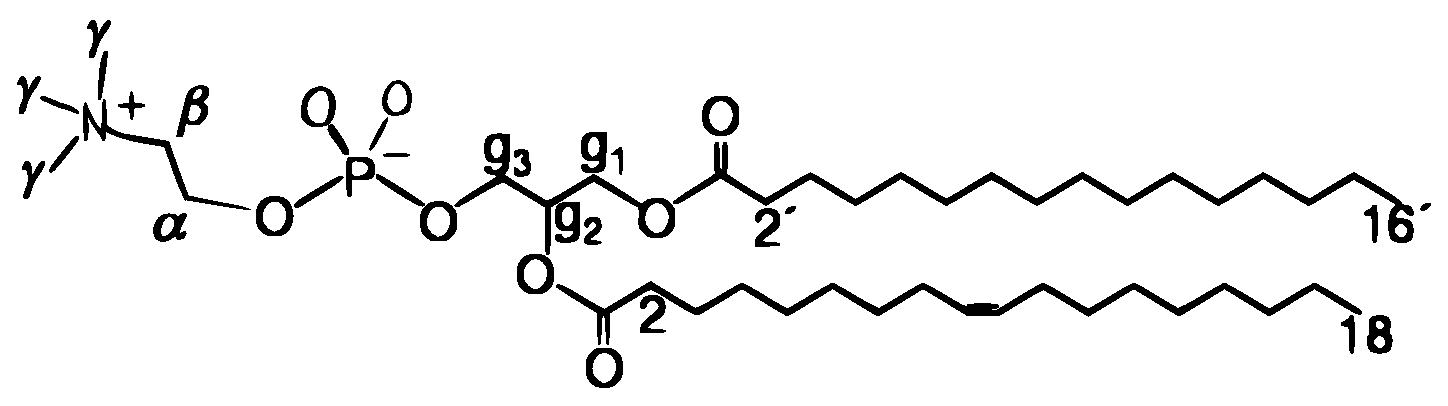
\includegraphics[width=7.5cm]{../Fig/POPCstructure.eps}
  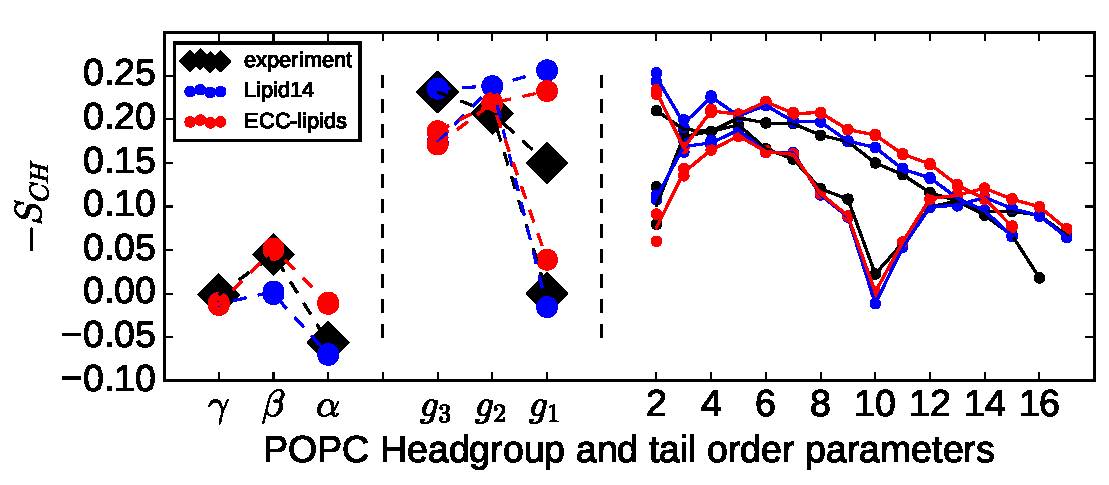
\includegraphics[width=8.0cm]{../Fig/ipython_nb/Order-parameters_exp-L14-ECCL17_q80_sig89.pdf}
  \includegraphics[height=8.4cm,angle=-90]{../Fig/form-f_exp-l14-eccl17.eps}
  \caption{\label{simVSexpNOions}
    Top: The chemical structure of POPC and the labeling of the carbon segments.
    Middle: Order parameters of POPC head group, glycerol backbone and acyl chains 
    from simulations with the Lipid14 \cite{dickson14} and the ECC-lipid models
    compared with the experimental values from \cite{ferreira13}.
    The size of the points for the head group order parameters correspond the
    of the error bars ($\pm 0.02$ for experiments \cite{botan15,ollila16} and ?? for simulations).
    The size of the points for acyl chains are decreased by a factor of 3 to improve the clarity of the plot.
    Bottom: X-ray scattering form factors from simulations with the Lipid14 \cite{dickson14} and
    the ECC-lipid models compared with experiments~\cite{Kucerka2011}.
  } 
  \todo{Increase the height of the order parameter figure} \\
  \todo{sn-1 and sn-2 order parameters should be somehow labelled in the order parameter figure. Maybe empty and filled points?} \\
  \todo{Add size of the error bars in simulations to the caption.} \\
  \todo{Would it be possible to increase the size of points for acyl chain order parameters only in z-direction such that
    it would correspond the error bars?} \\
  \todo{x-axis in form factor plot from 0 to 0.6, where experimental data ends. y-axis from 0 to $\sim$2.5 to remove the empty space.} \\
\end{figure}

\begin{table}
  \caption{Area per lipid (APL) values of POPC with no ions from the Lipid14 simulation
    ran in this work and from the literature, from ECC-lipid model and from experiments.\label{tab:apls} }
  \begin{tabular}{l|c c}
    model          & APL (\AA$^2$)   & Temperature [K] \\
    \hline
    Lipid14                   & 65.1$\pm$ 0.6  &  300 \\
    Lipid14 \cite{dickson14}  & 65.6$\pm$ 0.5  &  303 \\
    \hline
    ECC-lipids                & 62.2$\pm$ 0.6  &  300       \\
    \hline
    experiment \cite{jambeck12}\todoii{REF}{put original references, not Slipids param. paper.} & 64.3  &  303    \\
    \hline
  \end{tabular}
\end{table}


The ECC-lipid and Lipid14 models reproduce the experimental x-ray scattering form factors
of POPC bilayer with the similar accuracy in Fig.~\ref{simVSexpNOions}.
The area per lipid values from the Lipid14 model is slightly larger than the
experimental value in Table~\ref{tab:apls}, while the value from ECC-lipid model
is slightly smaller. Area per lipid values of the ECC-lipid model show some variation
when simulated with different water models in Table~\ref{tab:apls_si} (Supplementary Information),
however, all the values are close to the experimentally reported values.
In conclusion, the ECC-lipid model reproduces the experimental dimensions of POPC
lipid bilayer with the accuracy comparable to the other state of the art lipid models \cite{ollila16}.
%The optimal value for $f_\sigma$ was found by representing the overall membrane structure well
%by matching scattering form factors to experimental data~\cite{Petrache06, Kucerka08, Pabst10}.

The acyl chain order parameters of the Lipid14 model~\cite{dickson14} and the
ECC-lipid model agree with the experimental values with in the error bars
in Fig.~\ref{simVSexpNOions}, althought the ECC-lipid model gives slightly larger
values for {\it sn}-1 chain. Notably, the experimentally measured forking and
small order parameter values of $C_2$ segment in {\it sn}-2 chain are relatively well
reproduced by the both models. This has been suggested to indicate that the carbonyl
of {\it sn}-2 chain is directed towards the water phase, in contrast to the
carbonyl in {\it sn}-1 chain, which would orient more along the bilayer
plane~\cite{seelig75,schindler75,gawrisch92}. While this may be an important
feature for the ion binding details, it is not necessarily reproduced by the
available lipid models~\cite{ollila16}
%This is expected as the ECC model does not modify
%the already highly optimized parameters of this region in Lipid14. 

The order parameters of $\alpha$ and $\beta$ carbons in the headgroup are slightly larger
in the ECC-lipid model than in the Lipid14 model, which is apparently related to the
P-N vector orienting 7$^{\circ}$ more toward the water phase in the ECC-lipid model, 
see Fig.~\ref{OrderParameterCHANGESsurf}. With the current data we cannot,
however, conclude which one of the models give the more realistic
headgroup conformations. The ECC-lipid model gives
the $\beta$ carbon order parameter value closer to experiments, while
value for $\alpha$ carbon is better in the Lipid14 model.
Despite of some deviations from the experimental order parameter values
in Fig. \ref{simVSexpNOions},
the accuracy of the both models in the glycerol backbone region
is comparable to the other state
of art lipid models available in literature \cite{botan15}.


\todo{Dynamics check is missing: MSD (Hector/Joe)}

\subsection{Calibration of lipid electrometer:
            Response of POPC head groups to bound charge}\label{section:boundCHARGE}

\begin{figure}[tbp]
  \centering
  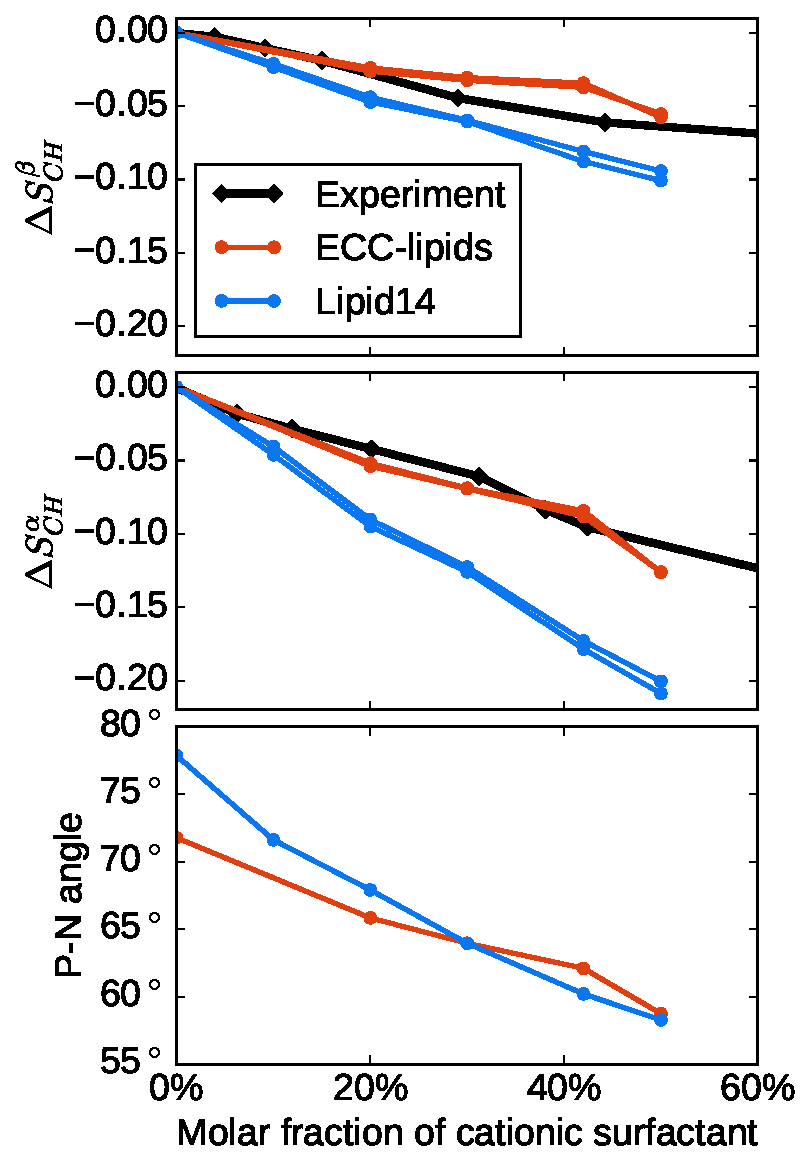
\includegraphics[width=8.0cm]{../Fig/ipython_nb/PN_angle_OrdPars-A-B_L14-ECCL17_q80_sig89_surf.pdf}
  \caption{\label{OrderParameterCHANGESsurf}
    The changes of headgroup order parameters and P-N vector orientation as a function of
    cationic surfactant (dihexadecyldimethylammonium) in POPC bilayer from simulations
    and experiments \cite{scherer89}.
  }
  \todo{Labeling should be consistent with the previous figure, i.e. experimental data with diamonds.} \\
  \todo{x-axis scale from -1 to 51 to make the point in zero fully visible and to remove empty space.} \\
  \todo{Empty space between figures and from the right column could be reduced.}
\end{figure}

Before proceeding to the ion binding affinity, we quantify
the response of the headgroup order parameters to the amount of 
bound charge by using mixtures of monovalent cationic
surfactants (dihexadecyldimethylammonium)
and POPC~\cite{scherer89}. The amount of bound charge per PC 
in these systems is given by the molar fraction of cationic 
surfactants, because essentially all surfactants with two hydrophopic
acyl chains can be assumed to locate in the lipid bilayers.
The experimental data for these systems can be used to validate 
the sensitivity of lipid headgroup order parameters
to the amount of bound charge in simulations.

The changes of the headgroup order parameters with an increasing amount of 
the cationic surfactant is compared between experiments~\cite{scherer89} and
simulations in Fig. \ref{OrderParameterCHANGESsurf}.
Approximately linear decrease of the order parameters, as expected from Eq. \ref{OPchangeEQ},
is observed in simulations and experiments at least for the mole fractions
below $\sim$30\%. The slope is, however, too steep in the Lipid14 model indicating that 
the head group order parameters respond too sensitively to the bound positive charge.
The slope in the ECC-lipid model is in very good agreement with experiments
for the $\alpha$ segment, while the slope is slightly
underestimated for the $\beta$ segment.

The headgroup P-N vector angle with respect to the membrane normal
is also shown in Fig.~\ref{OrderParameterCHANGESsurf}
as a function of the mole fraction of the cationic surfactant.
As suggested previously~\cite{seelig87}, the headgroup orients
more towards the water phase with the increasing amount of positive
charge in a PC lipid bilayer. The effect is more pronounced in the
Lipid14 model, for which the addition of 50\% mole fraction of the cationic
surfactant leads to the decrease of 20$^{\circ}$ of the P-N vector angle,
while the corresponding change in the ECC-lipid model is 11$^{\circ}$.
The difference is in line with the smaller order parameter 
changes and the reduced charge--dipole interactions in the latter model.
The lesser sensitivity of the P-N vector angle response in the ECC-lipid
model can be considered to be more realistic, because the changes of the headgroup
order parameters as a function of the bound positive charge
are in better agreement with experiments in this model.
The results also imply that the validation and improvements of MD simulation
models are generally required for the reliable simulation studies of the
lipid headgroup responses to ions or other biomolecules, as also concluded
previously \cite{botan15}.


%
%Therefore we use the data in Fig.~\ref{OrderParameterCHANGESsurf}
%to suggest a linear relation between $\alpha$-carbon order parameter
%and average P-N vector angle changes $\Delta \Theta_{\rm P-N}=?? \Delta S_{\rm CH}^{\alpha}$.
%This can be used to estimate the change in P-N vector angle
%from experiments measuring changes in $\alpha$-carbon order parameter. 
%\todo{SAMULI: I think that we should establish the relation between 
%order parameter and P-N vector angle changes by using ECC-lipids model.
%This would be useful for people measuring aplha order parameter
%changes from experiments.}
%
%For example, $\Delta S_{\rm CH}^{\alpha}=0.018$ measured due to the
%addition of 66.8 $\mu$M concentration of Mellittin in bulk water \cite{kuchinka89}
%gives $\Delta \Theta_{\rm P-N} = 2.5^{\circ}$.
%\todo{I looked this roughly from the figure, should be calculated from 
%the actual relation if we decide to put this.}


\subsection{Cation binding affinities to POPC membrane validated through lipid electrometer}

\begin{figure}[tbp]
  \centering
  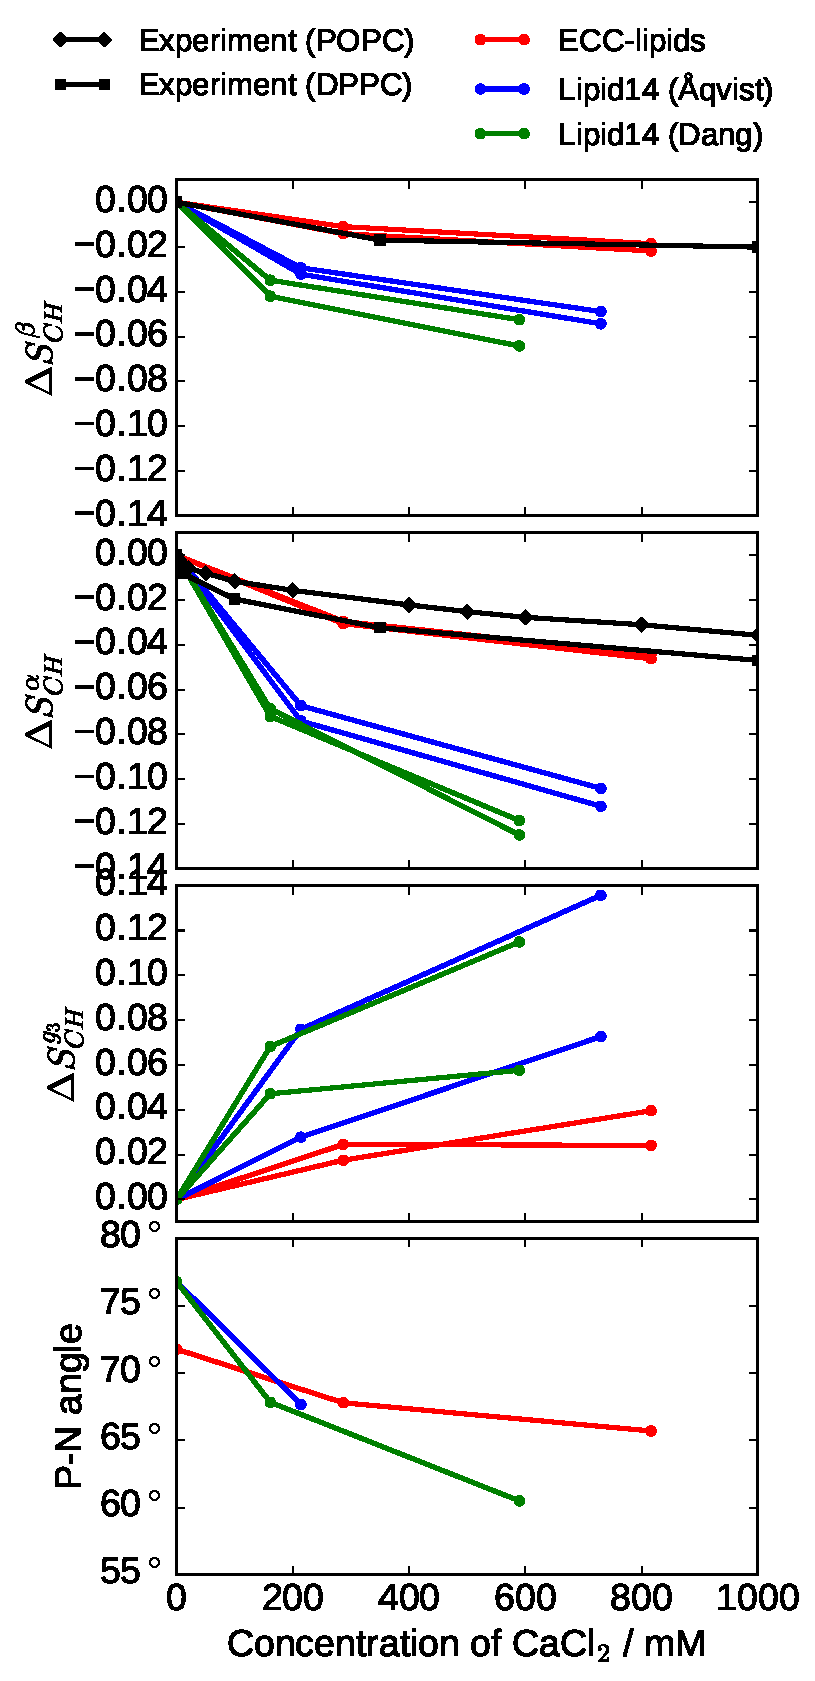
\includegraphics[width=8.0cm]{../Fig/ipython_nb/PN_angle_OrdPars-A-B-g3_L14-ECCL17_q80_sig89_CaCl.pdf}
  \caption{\label{fig:delta_ordPar_CaCl}
    Changes of head group order parameters of POPC bilayer as a function of CaCl$_2$ concentrations
    are shown from simulations with different force fields together with experimental data 
    (DPPC \cite{akutsu81} and POPC \cite{altenbach84}). 
    Ion concentrations in bulk water are shown in x-axis. 
    Values from simulations are calculated from the of cation number density $C_{np}$
    from the region at the simulatin box edge with the constant ion concentration as [ion]=$C_{np}/0.602$.
    Simulation data with Lipid14 and \AA{}qvist ion parameters is taken directly from Ref. \cite{catte16}.
  }
  \todo{I think that we must show the NaCl results in the main paper. I think that the best would
    be to use similar two column format, which we had before. This is used also in NMRlipids II and makes the
    comparison easier} \\
  \todo{The DPPC and POPC should be shown and properly labelled as we had previously.} \\
  \todo{The labeling should be consistent with previous figures, i.e., experiments with diamonds.} \\
  \todo{Start x-axis scale from -1 to make the point in zero fully visible.} \\
  \todo{Start y-axis scale of the two top figures from -0.13 to remove the empty space.} \\
  \todo{y-axis scale of the bottom figure from 59 to 78 to remove the empty space.} \\
  \todo{Empty space between figures and from the right column could be reduced.} \\
  \todo{Experimental values from \cite{akutsu81} to be put in the $g_3$ figure:
    the value of $g_3$ order parameter of DPPC was -0.214 
    in the absence of ions [average of two closely spaced splittings] and -0.211 in the presence
    of 0.35 M CaCl$_2$ (at 59 Celcius). No effect of ions could be detected on DPPC bilayers labeled
    at the C-2 segments of both fatty acyl chains.''
  }
\end{figure}

\begin{figure}[tbp]
  \centering
  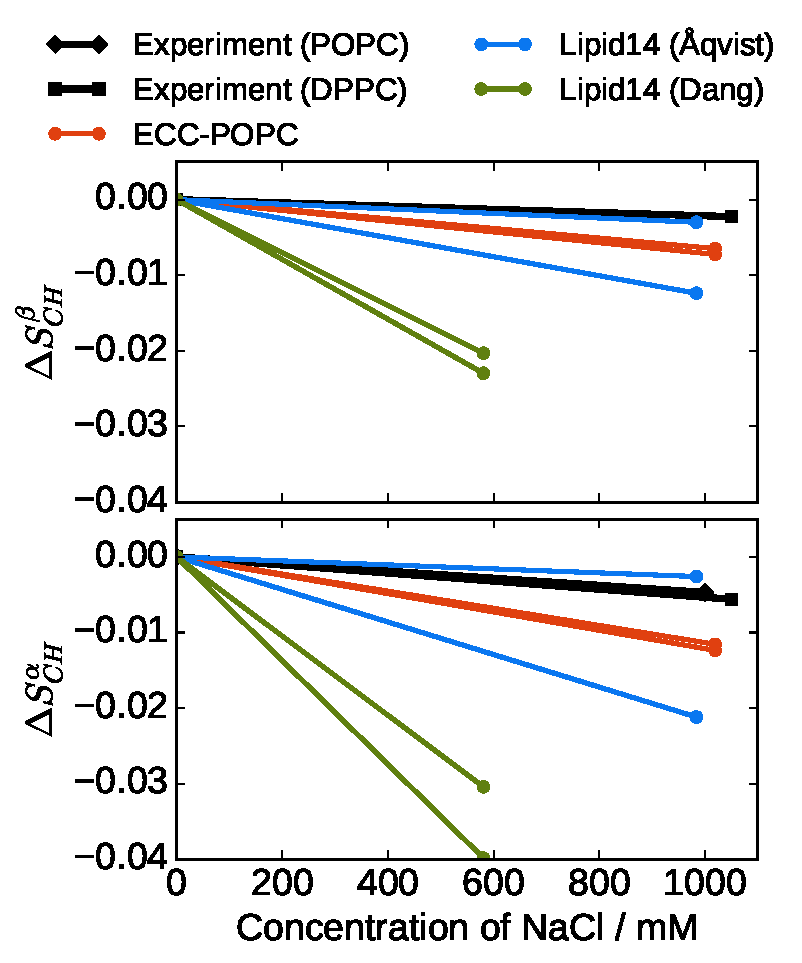
\includegraphics[width=8.0cm]{../Fig/ipython_nb/OrdPars-A-B_L14-ECCL17_q80_sig89_NaCl.pdf}
  \caption{\label{fig:delta_ordPar_NaCl}
    Changes of head group order parameters $\alpha$ and $\beta$ of POPC bilayer as a function of NaCl concentrations
    are shown from simulations with different force fields together with experimental data \cite{akutsu81}. 
    Ion concentrations in bulk water are shown in x-axis. 
    Values from simulations are calculated from the of cation number density $C_{np}$
    from the region at the simulatin box edge with the constant ion concentration as [ion]=$C_{np}/0.602$.
    Simulation data with Lipid14 and \AA{}qvist ion parameters is taken directly from Ref. \cite{catte16}.
  }
\end{figure}


The changes of the lipid bilayer headgroup order parameter from different simulations and
experiments \cite{akutsu81,altenbach84} are shown in Figs.~\ref{fig:delta_ordPar_CaCl} and~\ref{fig:delta_ordPar_NaCl}
as a function of NaCl and CaCl$_2$ concentrations.
%Responses to NaCl concentrations are in SI, Fig.~S\ref{fig:delta_ordPar_NaCl}.
These results can be used to compare the ion binding affinities to lipid bilayers
between simulations and experiments by using the electrometer concept, because 
the order parameters decrease proportionally to the amount of bound positive charge~\cite{seelig87,catte16}. 
The recent comparison of different simulation models to the experimental data
revealed that most models significantly overestimate the Na$^+$ ion binding to PC
lipid bilayers and that none of the available models correctly reproduce
the details of the binding of Ca$^{2+}$ ions \cite{catte16}.
A positive exception was the Lipid14 model \cite{dickson14} simulated with \AA{}qvist ions,
as seen from the data replotted from Ref.~\citenum{catte16} in Fig.~\ref{fig:delta_ordPar_CaCl}.
The model reproduced the experimentally measured small order parameter changes with NaCl
and imperceptible Na$^+$ binding to PC bilayers \cite{akutsu81,altenbach84}.
However, the changes of the headgroup order parameters as a function of CaCl$_2$ 
concentration were overestimated by the same combination of force field parameters.

Since significant artefacts are reported in simulations with \AA{}qvist ions is water \cite{??},
we also simulated the Lipid14 model with the ion models by Dang et al.~\cite{smith94,chang1999,dang2006} and
ECC-ions~\cite{jungwirth17-new-paper-to-be-published, kohagen16, Pluharova2014} having
more realistic bulk behaviour. Instead of the improvement in the binding behaviour,
we observed overbinding also of Na$^+$ with these ions models, while the results
with Ca$^{2+}$ were barely affected,
%for the CaCl$_2$ interactions with a POPC bilayer described by the Lipid14 model,
as seen in Figs. \ref{fig:delta_ordPar_CaCl} and S??.%\ref{fig:ordPars_waterModels} (in SI), respectively.
\todo{Add OP-response of Lipid14+ECC-ions plot in SI}.
The results are in line with the previous work \cite{catte16},
suggesting that the improvements in the lipid parameters are
required to correctly describe the divalent cation binding to PC lipid bilayers.

%To improve the cation binding behaviour to POPC lipid bilayer we implicitly included the electronic
%polarization to the Lipid14 model by using the ECC approach as described in section \ref{section:ecc}.
Our simulations with the ECC-lipid and the ECC-ion models \cite{jungwirth17-new-paper-to-be-published, kohagen16, Pluharova2014}
exhibit an improved behaviour of cation binding to a POPC bilayer
showing a good agreement with experiments in the changes of 
the lipid headgroup order parameters as a function of NaCl and CaCl$_2$ concentrations
in Fig.~\ref{fig:delta_ordPar_CaCl}. Since also the headgroup order parameter
response the to the bound positive charge the ECC-lipid model
was in good agreement with experiments in section \ref{section:boundCHARGE},
we conclude that the model correctly reproduces the binding affinity of
Na$^{+}$ and Ca$^{2+}$ ions to POPC lipid bilayer.
%In conclusion, the results suggest that 
%the ECC-lipid model together with the ECC-ion parameters gives a realistic
%description for the binding affinities of Na$^+$ and Ca$^{2+}$ ions to POPC lipid bilayer. 
Furthermore, the overestimated headgroup order parameter changes of POPC in the Lipid14
model as a function of CaCl$_2$ concentration arise from both, the overestimated
binding affinity and sensitivity of the headgroup tilt to the bound positive charge.
This probably applies also to the other lipid models considered in the previous study~\cite{catte16},
emphasizing the importance of the comparison of the lipid headgroup order parameter response
to the bound charge between simulations and experiments as done in section \ref{section:boundCHARGE}.

\todo{SAMULI: Maybe we should discuss the repeat distances and
  area per molecules measured at \cite{petrache06,pabst07,uhrikova08}
  }





\subsection{Cation binding to POPC membrane in atomistic detail}

To quantify the binding affinities in different models we calculated 
the relative surface excess from Eq.~\ref{surfexcess}. 
Calcium cations at a molar concentration of $350\,\mathrm{mM}$ provide
$\Gamma_i^w = 0.07 \pm 0.01 \rm{nm}^{-2}$ in the ECC-lipid model, which is significantly
smaller than the values for the Lipid14 model with \AA{}qvist ions, $\Gamma_i^w = 0.13 \pm 0.01 \rm{nm}^{-2}$,
or with Dang ions, $\Gamma_i^w = 0.3 \pm 0.03 \rm{nm}^{-2}$.
\todo{JOE: I'd put the $\Gamma$ values into a table}
Interestingly, the relative surface excess of 
\ce{NaCl} at $1\,\mathrm{M}$ concentration (ECC-ions~\cite{Pluharova2014}) is qualitatively different from \ce{CaCl2}
having a negative value $\Gamma_i^w = -0.1 \pm 0.01 \rm{nm}^{-2}$, 
meaning that water molecules are preferred to sodium and chloride ions at the membrane-water interface. 
This is in contrast to previous works employing classical MD simulations,
which generally agree together on the existence of an increased sodium density at the membrane-water interface.
\todo{JOE: Add references to NaCl simulation papers that show peaks.
Add a simple note that there is NBFIX trick in Charmm36 (?).} 
This finding is depicted in Figures~\ref{fig:nacl-dens} and~\ref{fig:cacl-dens},
which show the density profile of ions and water along the membrane normal. 
%The density profiles show
%a larger Ca$^{2+}$ density peak in lipid headgroup region for
%the Lipid14 model with Dang and ECC-ions than for the ECC-lipid model.
\todo{Densities and relative surface excess from NaCl systems to be added.
  The discussion below to be finished after this.}


\begin{figure}[tbp]
  \centering
  \includegraphics[width=9.0cm,angle=0]{../Fig/CAdensities2.eps}
  \caption{\label{fig:cacl-dens}
    Number density of \ce{Ca^{2+}} and \ce{Cl^-} as a function of membrane normal axis
    for different force fields. Data for Lipid14 with \AA{}qvist ions are taken directly from Ref. \citenum{catte16}.
    %Normalization factor for ions is 1 for monovalent ions (i.e.~\ce{Na^+} and~\ce{Cl^-}),
    Densities of~\ce{Cl^-} and water are divided with 2 and 200, respectively, to visalize them
    with the same scale as \ce{Ca^{2+}}. The molar concentration of the ions in water is 350~mM in all systems
    presented here. 
    }
  \todo{PAVEL: draw phosphate position with its variance, add water density (scaled) and include the number of$\Gamma$-surface access.} \\
  \todo{JOE: Change the figure so that it contains a membrane background} \\
\end{figure}


We can estimate relative binding affinities 
of several moieties in POPC towards \ce{Ca^{2+}} and \ce{Na+} cations 
using the number of contacts per lipid between cations and POPC oxygen atoms, 
$\Sigma ^\mathrm{Na^{2+}} _\mathrm{O}$,
in which a contact between the two atoms is counted 
if their distance is less than or equal $0.3 \, \mathrm{nm}$ 
(robustness of this definition discussed in reference~\citenum{javanainen17}). 

For sodium at $1000\,mM$ concentration 
the average number of contacts per lipid with any oxygen atom in POPC is 
$\Sigma ^\mathrm{Na^{+}} _\mathrm{O} = 0.106 $,    % = 17.1/128 
whereas if only phosphate oxygen atoms are considered 
this number decreases to 
$\Sigma ^\mathrm{Na^{+}} _\mathrm{PO_4} = 0.085 $,    % = 17.0/128 . 
and if only carbonyl oxygen atoms are counted 
it is even lower, 
$\Sigma ^\mathrm{Na^{+}} _\mathrm{O_{carb.}} = 0.048 $.    % = 4.3/128 . 
This means that interaction of sodium and POPC 
has balanced contributions of 55\% from only phosphate oxygens 
(i.e. no contacts with carbonyl oxyens),
and from only carbonyl oxygens with 20\% of configurations 
leaving 25\% for mixed phosphate and carbonyl oxygen configurations.  
This is in line with the calculated negative value of 
relative surface excess of sodium with respect to water, $\Gamma_i^w$, and
their density profiles along the membrane normal (Fig.~\ref{fig:nacl-dens})
suggesting that the populations of bound sodium cations 
naturally decrease with the decreasing density of water. 

In contrast to sodium, the dominant contribution
to the binding of \ce{Ca^{2+}} to POPC membranes comes from the phosphate group. 
% Numbers from simulation with 346mM conc. CaCl2
The average number of contacts per lipid 
between \ce{Ca^{2+}} at $290\,\mathrm{mM}$ concentration and any oxygen atom in POPC is 
$\Sigma ^\mathrm{Ca^{2+}} _\mathrm{O} = 0.134 $,    % = 17.1/128 
whereas if only phosphate oxygen atoms are considered 
the average number of contacts decreases only by a tiny amount to 
$\Sigma ^\mathrm{Ca^{2+}} _\mathrm{PO_4} = 0.133 $,    % = 17.0/128 . 
and if only carbonyl oxygen atoms are considered 
%(phosphate oxygens contribute, but are not counted as contacts),
this value is merely
$\Sigma ^\mathrm{Ca^{2+}} _\mathrm{O_{carb.}} = 0.033 $.    % = 4.3/128 . 
% Numbers from simulation with 980/845mM conc. CaCl2
%The average number of contacts per lipid between \ce{Ca^{2+}} and any oxygen atom in POPC is 
%$\Sigma ^\mathrm{Ca^{2+}} _\mathrm{O} = 0.264 $,    % = 33.8/128 
%whereas if only phosphate oxygen atoms are considered 
%the average number of contacts decreases only by a tiny amount to 
%$\Sigma ^\mathrm{Ca^{2+}} _\mathrm{PO_4} = 0.262 $,    % = 33.5/128 . 
%and if only carbonyl oxygen atoms are considered 
%(phosphate oxygens contribute, but are not counted as contacts),
%this value is merely
%$\Sigma ^\mathrm{Ca^{2+}} _\mathrm{O_{carb.}} = 0.066 $.    % = 8.4/128 . 
Hence, calcium is in contact with phosphate oxygens for 99\% of the time it is bound to the membrane, 
whereas only 25\% of the time accounts for contacts with carbonyl oxygens,
and interactions purely with carbonyl oxygens account for less than 1\% of configurations. 
Higher concentration of \ce{CaCl2} naturally increases the amount of contacts per lipid,
for $850\,\mathrm{mM}$ concentration of \ce{CaCl2}
the average number of contacts per lipid is increased to
$\Sigma ^\mathrm{Ca^{2+}} _\mathrm{O} = 0.264 $, 
but the distribution of states between phosphate and carbonyl oxygens remains unchanged. 
We corroborate this finding with the probability isodensity contours in Fig.~\ref{fig:volmaps}, 
and density profiles of ions and water along the membrane normal in Fig.~\ref{fig:cacl-dens}. 



\begin{figure}[tbp]
  \centering
  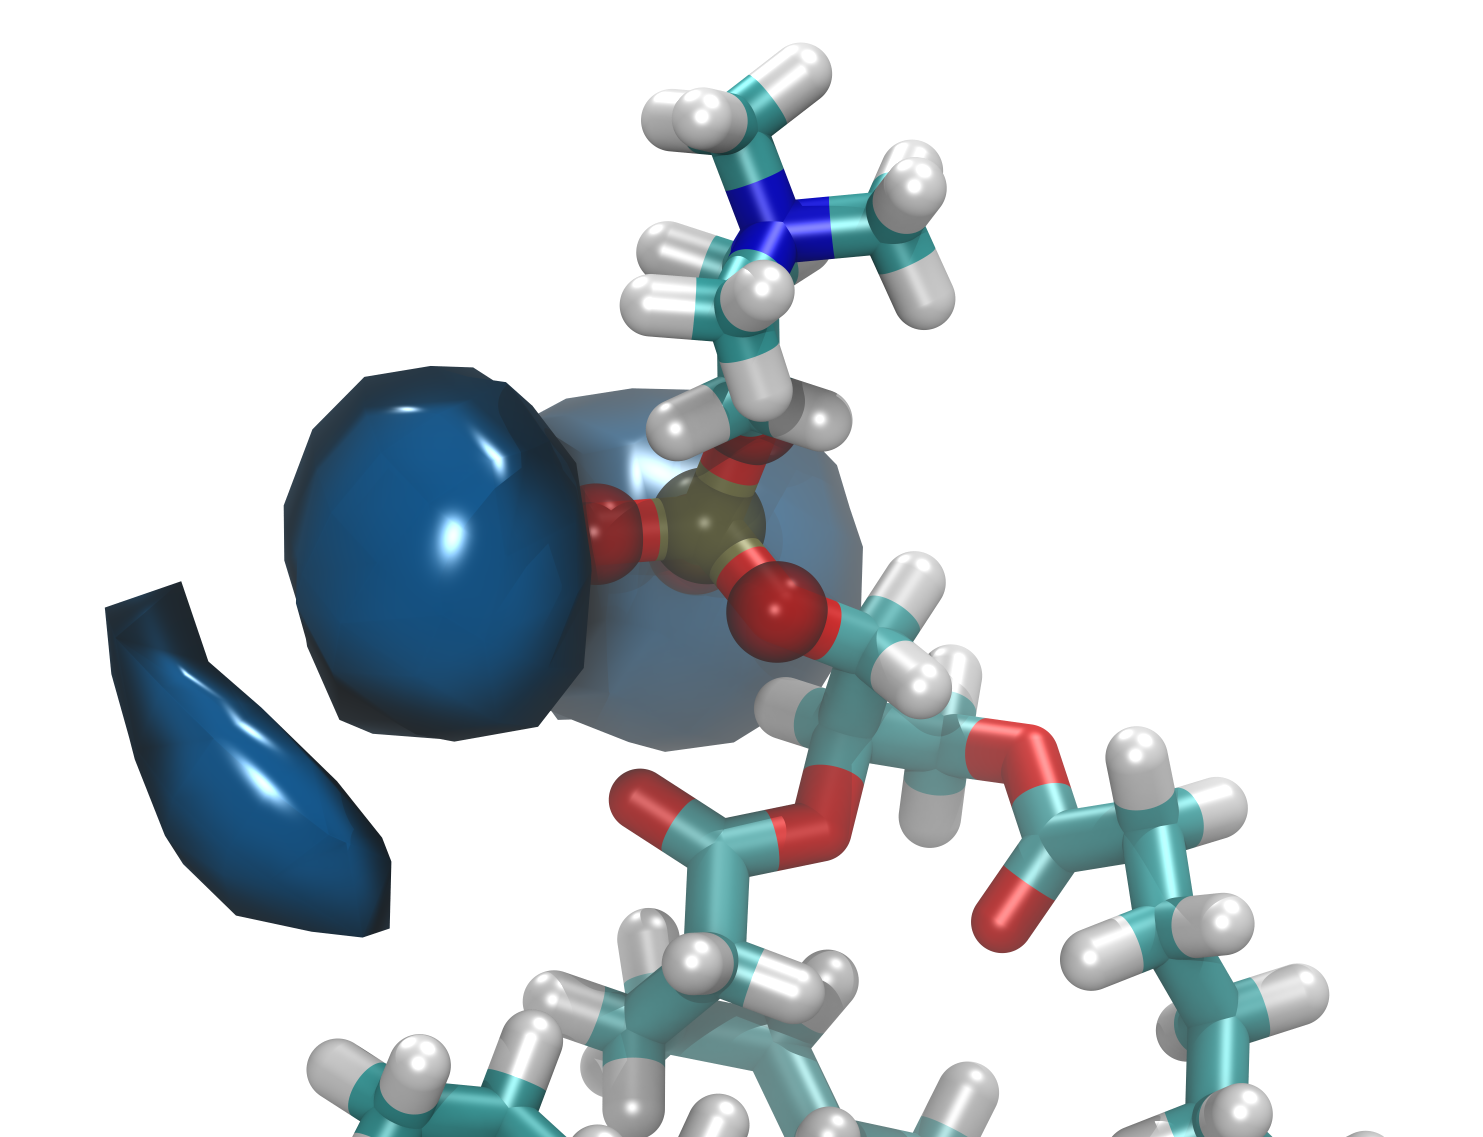
\includegraphics[width=6.0cm]{../Fig/volmap_resid10_Ca_Cl_PO4Cent.png} \\
  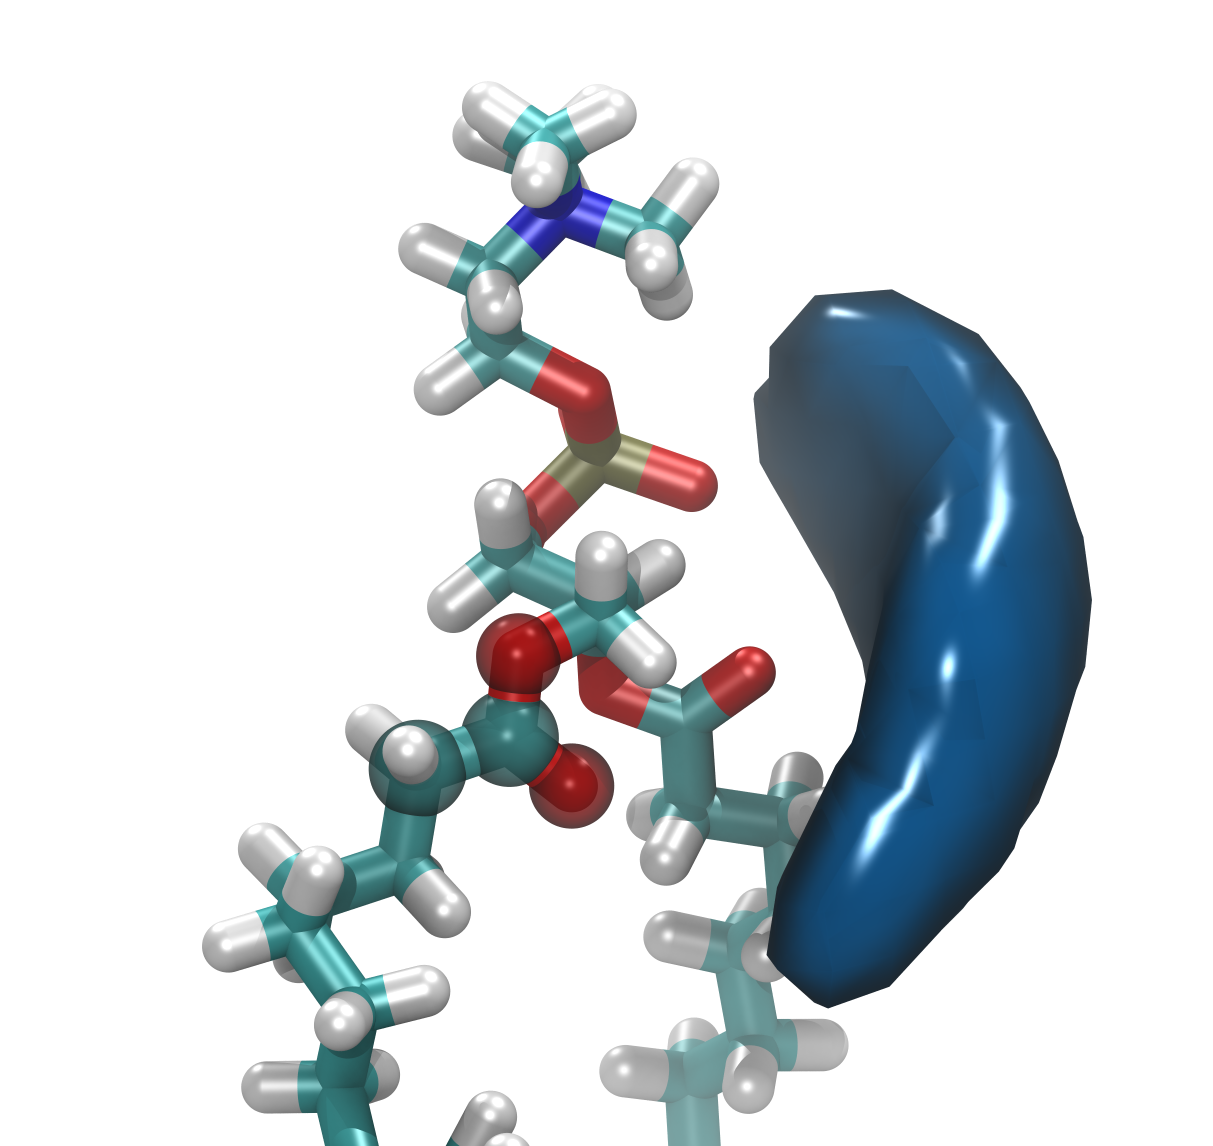
\includegraphics[width=4.0cm]{../Fig/volmap_resid10_Ca_Cl_sn1Cent.png}
  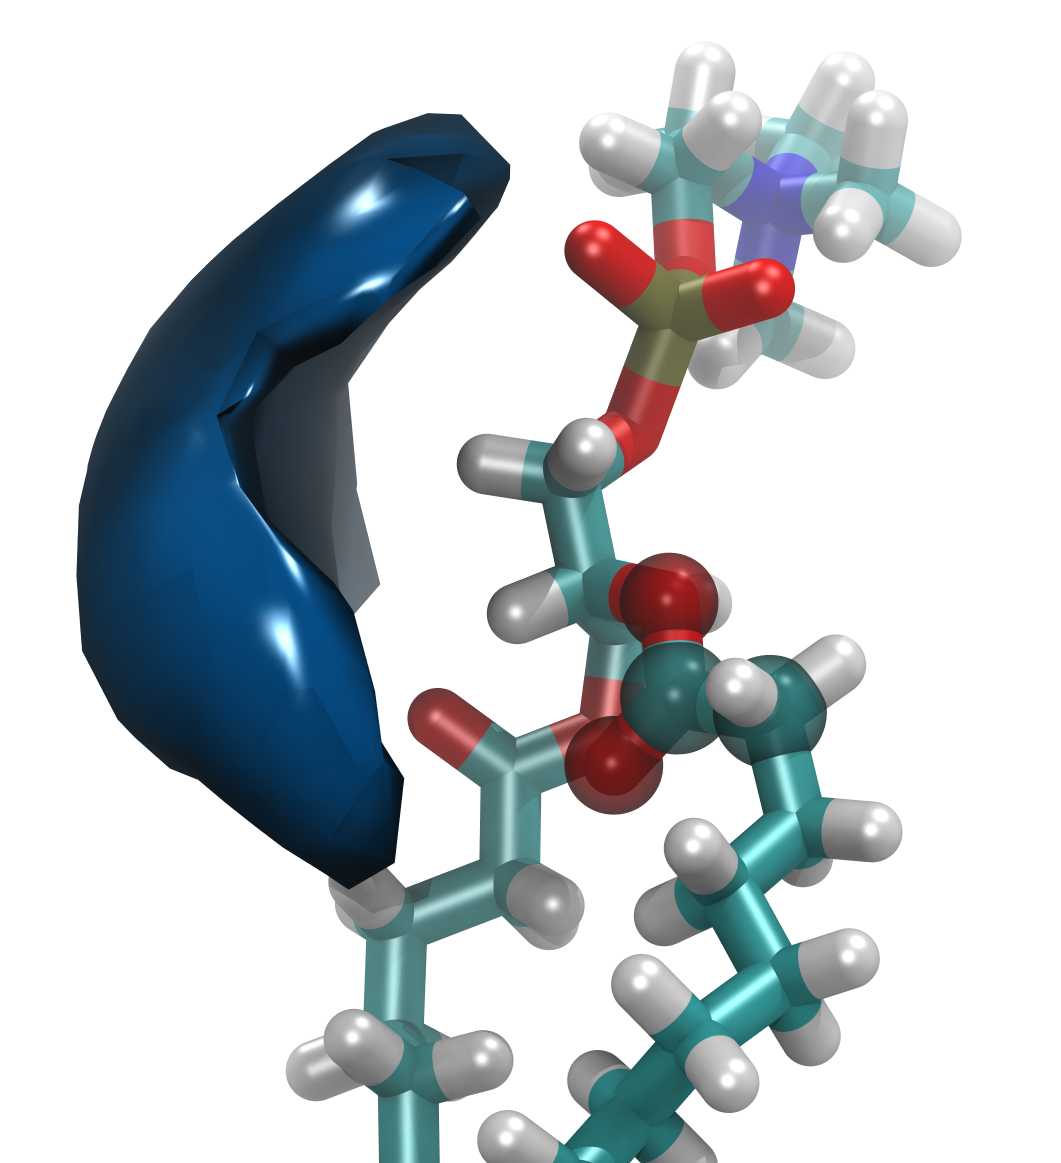
\includegraphics[width=3.6cm]{../Fig/volmap_resid10_Ca_Cl_sn2Cent.png}
  \caption{\label{fig:volmaps}
      Contours of probability isodensities of \ce{Ca^{2+}} with respect to 
      various moieties fixed in space (highlighted with transparent spheres): 
      phosphate moiety, side chain 1 carbonyl group and side chain 2 carbonyl group.
      Shown contours suggest that the dominant contribution 
      to \ce{Ca^{2+}} binding comes from the phosphate oxygens,
      whereas the interactions with any of the two carbonyl groups are considerably milder.
  }
  \todo{JOE: I'll update this figure with some ensemble of configuration to support binding preference of \ce{Ca^{2+}}}
\end{figure}



\subsection{Residence times of \ce{Na+} and \ce{Ca^{2+}} cations in POPC membrane}

The residence time of \ce{Ca^{2+}} in a POPC membrane 
is experimentally estimated to be lower than $10\,\mu\mathrm{s}$~\cite{altenbach84}. 
From a recent theoretical work with long simulations \cite{javanainen17}
this time can be roughly estimated 
in the order of $1\,\mu\mathrm{s}$~\cite{javanainen17}. 
Based on Fig. S17 in that work, Ref.~\citenum{javanainen17},
we took the simulation with the apparent highest fluctuations of the number of bound calcium,
which can be obtained at \url{https://doi.org/10.5281/zenodo.259376}
and anaylsed the residence times.
% simulation: (Matti C36 with CaClMK, 800ns total):
We find out that
approximately 20\% of bound residence times of \ce{Ca^{2+}} 
are limited by the length of the simulation, $800\,\mathrm{ns}$, 
and only less than
60\% of bound residence time is smaller than half of the simulation length , $400\,\mathrm{ns}$. 
Other simulations reported in that work show even longer residence times. 


This is in contrast to our model, ECC-lipids, 
which estimates the residence time of calcium bound to a POPC membrane to be 
smaller than $60\,\mathrm{ns}$ for 90\% of the time a cation is bound. % exactly $53\,\mathrm{ns}$
i.e. at least two orders of magnitude lower than previous estimates.
In addition, the longest observed residence time in our simulation is $120\,\mathrm{ns}$, 
which is well below the length of our simulations.
This is unfortunately not the case of many theoretical works,
where the residence time cannot be estimated,
or the simulation has not even decorrelated from it's 
initial condition with a population of bound/unbound cations \cite{catte16}, 
because it is limited by the simulation length, 
even though it can be very long (order of $\mu\mathrm{s}$) in some works, e.g. reference~\citenum{javanainen17}. 
Increasing time scales to the order of $\mu\mathrm{s}$ 
doesn't help to alleviate such a problem in current lipid models \cite{javanainen17}. %and also \cite{catte16}, but same simulation was used. 
Such a finding changes the point of view on binding of calcium to PC membranes from
a very strong long-term stable binding with rare exchanges to 
a relatively frequent exchange of clacium cations 
in equilibrium between membrane and solvent. 

Interestingly, \ce{Na+} cations exhibit much more rapid exchange between membrane and solvent than calcium.
The residence time of sodium bound to a POPC membrane is
smaller than $2\,\mathrm{ns}$ for 90\% of the time it is bound to the membrane 
with the longest measured bound time being $13\,\mathrm{ns}$. 
Such an exchange between membrane and solvent 
is an order of magnitude faster than for calcium cations. 
A histogram of residence times from our simulations is in Fig.~S\ref{fig:hist_residence_times} in SI. 
\todo{JOE: Plot a histogram of residence times based on our simulations and simulation from \citenum{javanainen17} and put it into SI.
 }

\subsubsection{Internal side-note: }
However, $\Sigma ^\mathrm{Ca^{2+}} _\mathrm{O_{carb.}}$ is increased 
in simulation withy the highest \ce{CaCl2} concentration
when carbonyl dipoles are scaled only with 0.945 
(roughly done through charge redistribution)
 to : $\Sigma ^\mathrm{Ca^{2+}} _\mathrm{O_{carb.}} \approx 0.08 $.    % = (70.-59.8)/128 . 

The average number of contacts per lipid between \ce{Ca^{2+}} and any oxygen atom in POPC is 
$\Sigma ^\mathrm{Ca^{2+}} _\mathrm{O} = 0.264 \rightarrow 0.309 $,
whereas if only phosphate oxygen atoms are considered 
the average number of contacts decreases only by a tiny amount to 
$\Sigma ^\mathrm{Ca^{2+}} _\mathrm{PO_4} = 0.262 \rightarrow 0.303 $,    % = 33.5/128 . 
and if only carbonyl oxygen atoms are considered 
(phosphate oxygens contribute, but are not counted as contacts),
this value is merely
$\Sigma ^\mathrm{Ca^{2+}} _\mathrm{O_{carb.}} = 0.066 \rightarrow 0.139 $.    % = 8.4/128 . 

This means that calcium is in contact with a phosphate oxygen for 98\% of the time it is bound to the membrane, 
whereas 46\% of the time accounts for contact with a carbonyl oxygen,
and purely carbonyl bound states account for less than 2\% of configurations. 
The states that have a contribution from carbonyl oxygens also contain a bound phosphate, 
so it can be thought of rather as a stabilizing moiety. 

The residence times change to 75ns (90\% of bound time) and max is 185ns.
That's not much, too. It certainly is not a game changer, I'd even call it to be within accuracy. 
The slight problem may be that with this tweak, there's approx. 17\%  more cations bound to the membrane,
which means, I'd need to tune the sigma parameter a bit (increase the scaling factor $f_\sigma$). 
That could detune the membrane structure \dots
Not $f_q$ -- that's set by the simulations with the surfactant. Good.
I think that such a binding detail is within the accuracy of the proposed simple correction.
It would be worth noting that the model may underestimate slightly the contribution from carbonyls due to this. 
But we can't say to what extent\dots



%\begin{figure}[tbp]
%  \centering
%  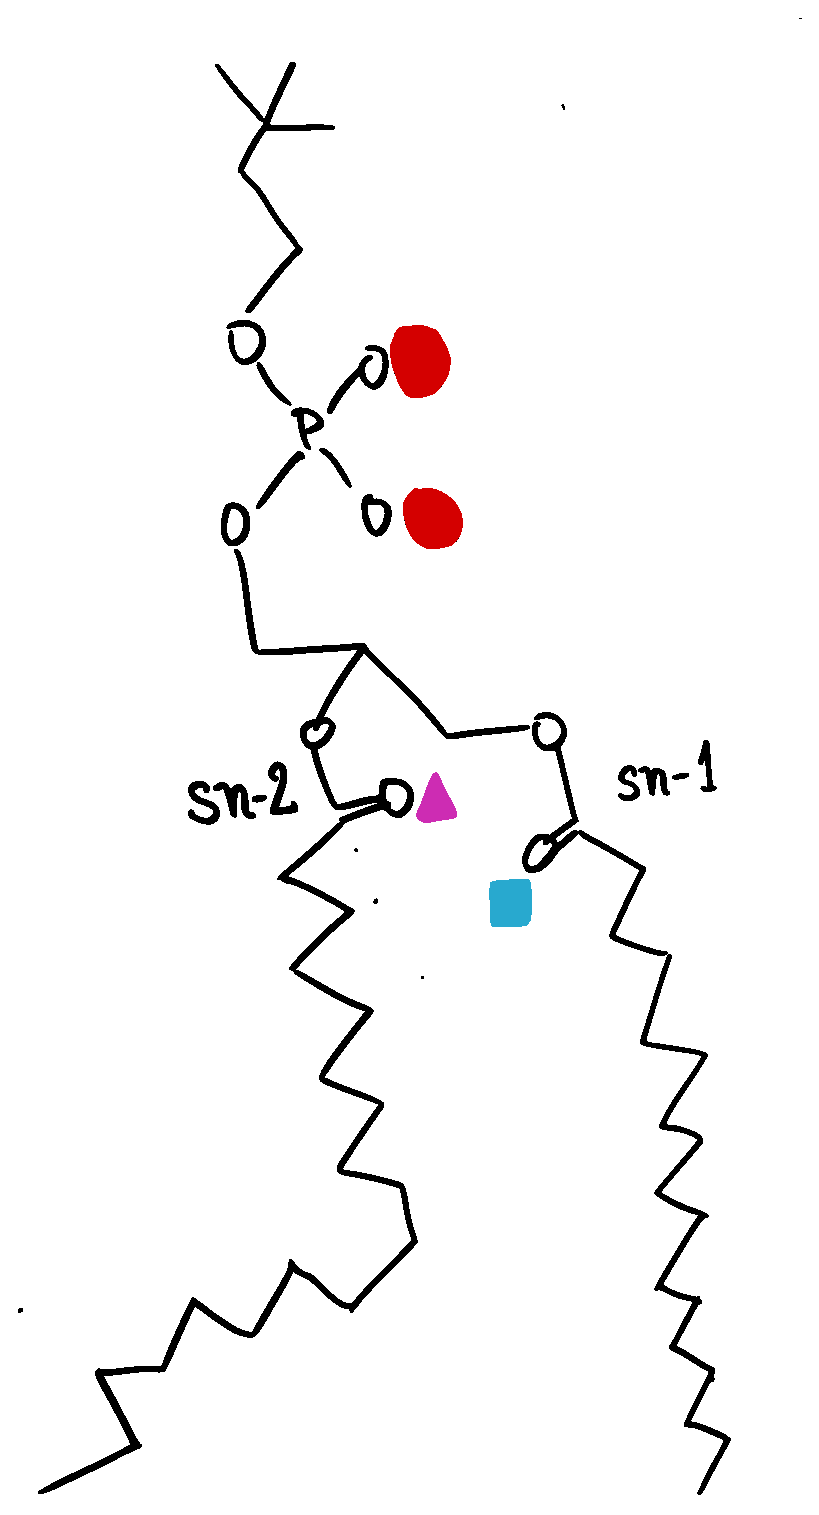
\includegraphics[height=6.0cm]{../Fig/POPC_binding_labels.eps} 
%  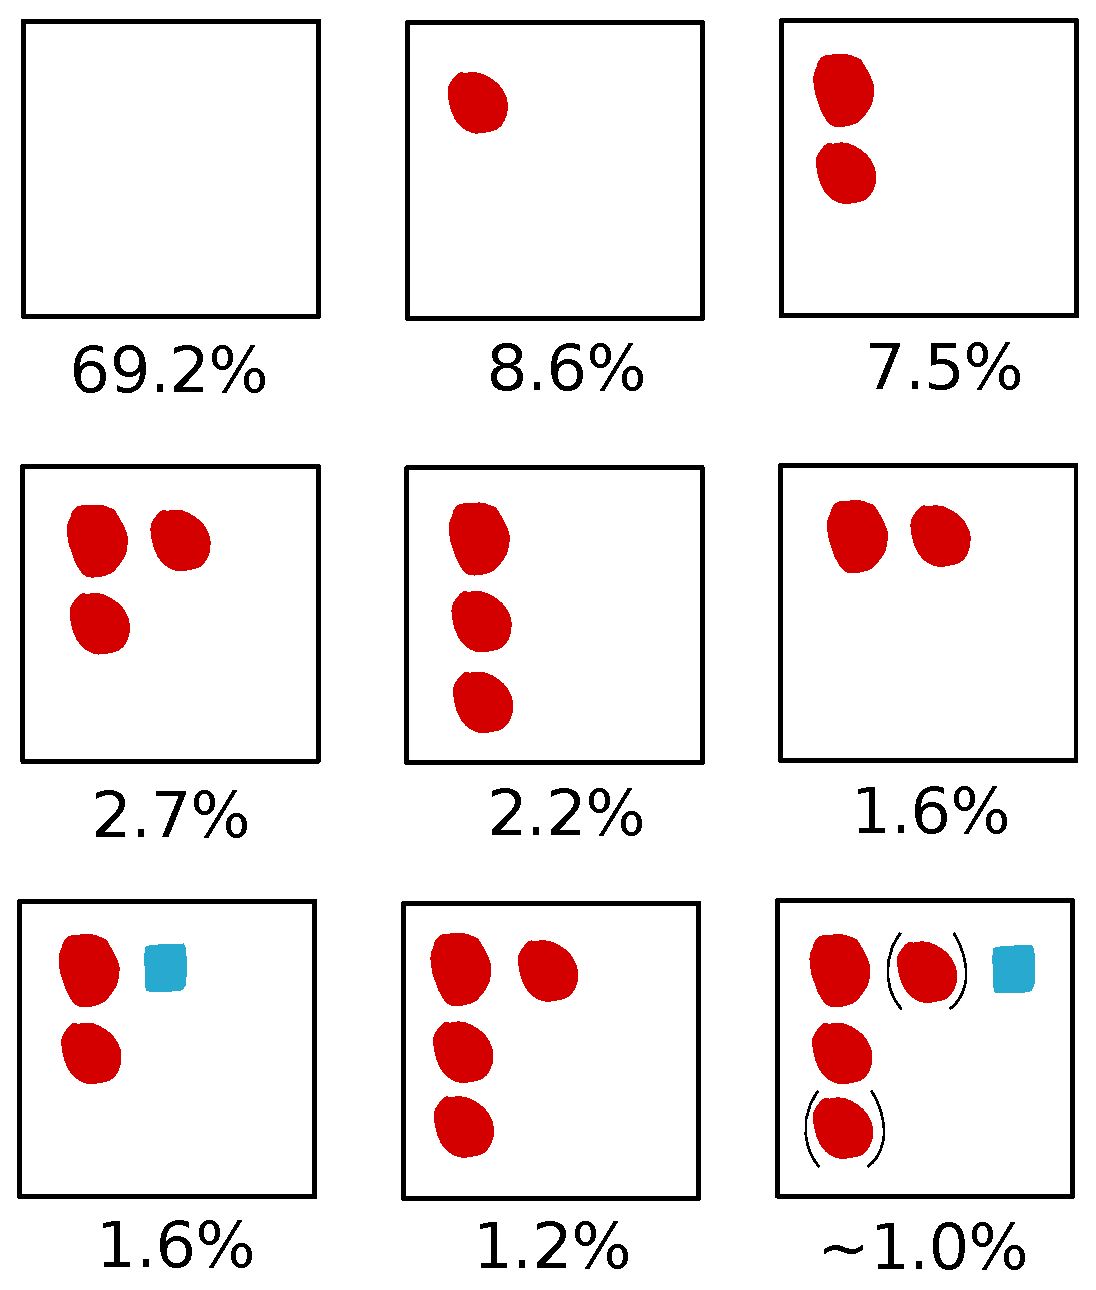
\includegraphics[height=6.0cm]{../Fig/POPC_binding_ECC-lipids.eps}
%  \caption{\label{fig:binding_conf}
%      Configurations of \ce{Ca^{2+}} binding in POPC membranes in the ECC-lipids model.
%      The binding sites are: 
%      red circle for phosphate oxygens; 
%      blue square for sn-1 carbony oxygen; and green triangle for sn-2 carbonyl oxygen.
%      The configurations along with their probabilities are drawn in the following manner:
%      each row corresponds to an individual lipid the cation is bound to;
%      symbols denote the site the cations is bound to the respective lipid.
%      An empty configuration denotes an unbound cation in a solvent. 
%  }
%\end{figure}





\subsection{Stoichiometry of binding of \ce{Na+} and \ce{Ca^{2+}} cations to POPC membrane}

%Binding probability:
%\ce{Ca2+} complex with \\
%1 POPC - 13\% -- 30\% \\
%2 POPC - 18\% -- 42\% \\
%3 POPC - 12\% -- 28\% \\

Simulations allow us to directly evaluate the stoichiometry 
by calculating relative propensities of various \ce{Ca^{2+}}:$n\times$POPC complexes
by evaluating contacts between cations and lipids with a cut off radius $0.3\,\mathrm{nm}$. 
The propensities of \ce{Ca^{2+}}:$n\times$POPC complexes at 285~mM concetration 
are in order:
$42\%$ for two lipids,
$30\%$ for one lipid, and
$28\%$ for three lipids.
Apart from a ternary complex, in which one calcium cation binds two lipids, 
we also find complexes with 1~and 3~lipids
occuring with only a slightly lower but similar probability
as shown in Figure~\ref{fig:cacl_complexes}. 

\begin{figure}[tbp]
  \centering
  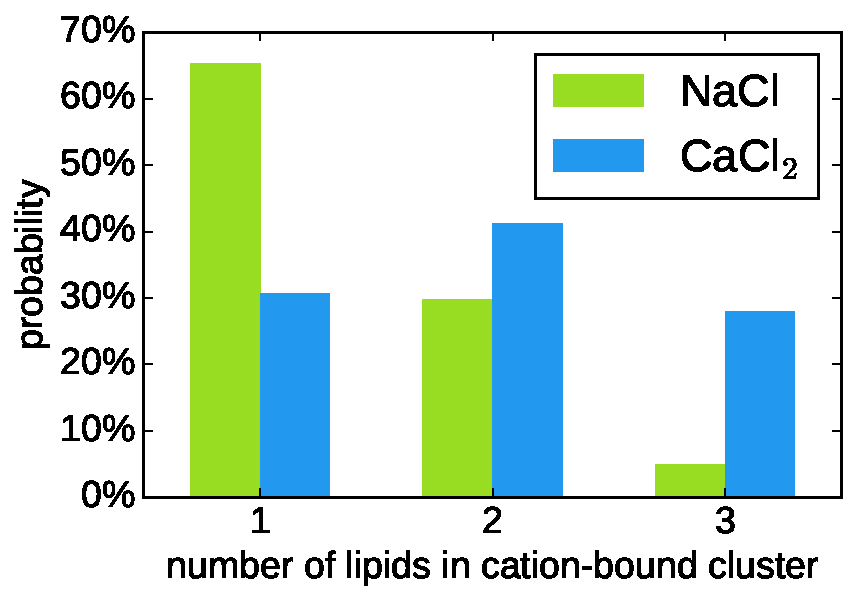
\includegraphics[width=6.0cm]{../Fig/ipython_nb/stoichiometry_NaCl-CaCl2_comparison_Ecc-lipids.pdf} \\
  \caption{\label{fig:cacl_complexes}
      Relative probabilities of existence of \ce{Na^{+}} or \ce{Ca^{2+}} complexes
      with a certain number of POPC lipids. 
      \ce{Na^{+}} complexes were evaluated from the simulation with 1~M concentration;
      and \ce{Ca^{2+}} complexes were evaluated from the simulation with 287~mM concentration.
  }
\end{figure}

Several binding models were proposed and tested~\cite{altenbach84} of which only one,
ternary complex binding model, provided a good fit of the experimental observations. 
In such a model, it is assumed that \ce{Ca^{2+}} cations bind to a POPC membrane 
with a stoichiometry 2~POPC:1~\ce{Ca^{2+}}.
In a later work~\cite{macdonald87}, 
a Langmuir adsorption model (i.e. stoichiometry 1~POPC:1~\ce{Ca^{2+}}) 
was found to provide as good fit as ternary complex model, 
when only low concentrations of \ce{CaCl2} are considered.
Ternary complex model also provides a good fit 
to our simulations with ECC-lipids 
(see Fig.~\ref{fig:cacl-bind} in SI and its caption for details). 
The symmetry of the distribution of complexes from simulation 
as shown in Figure~\ref{fig:cacl_complexes} --   
i.e. almost equal probabilities of complexes with 1 or 3 lipids 
that behave in the total average picture as complexes with 2 lipids -- 
provides clues why ternary complex binding model 
fits both simulation and experimental results relatively well, 
although it is apparently incorrect. 
It is also worth noting that many binding constants in the literature
(e.g., Marsh's handbook \cite{marsh13}) 
are based on the headgroup order parameter changes 
intepreted with the ternary complex binding model. 

\todo{SAMULI: I think the we should make clear that the current binding
  constants in, e.g., Marsh's handbook are based on the headgroup order parameter
  changes intepreted with ternary complex binding model. I.e. the experimental raw data
  is excatly the same as we have in this work. Our simulations enable much more versatile interpretation
  of the binding phenomena. I think that this is one the main points of this work, so this comment
  applies to the previous section, introduction, abstract and conclusions as well.
  JOE: agree, this would be a good statement in general. I'll try to put it into the text.
}

Binding of \ce{Na+} cations to a POPC membrane 
mostly follows stoichiomtetry \ce{Na^{+}}:$1\times$POPC 
as shown in Figure~\ref{fig:cacl_complexes}. 




\section{Conclusions}

By using the electrometer concept we show that the binding of \ce{Na^+} and \ce{Ca^2+} ions
to a POPC lipid bilayer can be accurately described with the classical MD simulation 
force field, where the electronic polarization is implicitly included using 
the electronic continuum correction (ECC)~\cite{leontyev11}.
The proposed ECC-lipids model is a significant improvement over 
other available lipid models, which all overestimate specific cation binding affinities~\cite{catte16}.  
While the structural details of a POPC lipid bilayer simulated with the ECC-lipids
model agree with experiments with the comparable accuracy to the other state of the art lipid models,
it also reproduces the experimental lipid head group order parameter responses to
the cationic surfactant, NaCl and CaCl$_2$ concentrations. 

The good agreement with experiments enables the atomic resolution 
interpretation of NMR experiments by using MD simulations.
In agreement with previous interpretations of experimental data \cite{hauser76,hauser78,herbette84,binder02},
the Ca$^{2+}$ ions mainly interact with phosphate oxygens.
However, the stoichiometry of the binding is significantly more complicated 
than in the previous interpretation of the NMR data based on 
the ternary complex model, where one calcium binds to two POPC molecules~\cite{altenbach84}.
The complexes of one calcium bound to two lipids are the most probable also in the
ECC-lipids model, but the complexes of one or three lipids per one calcium
were observed to be almost equally likely. While the success of the ternary
compex model is understandable based on the simulation results,
a simple binding model cannot detec the complex binding
oberved in the simulation.

The improved cation binding behaviour to POPC bilayer pave the way for
simulations of complex biochemical systems with correctly described
electrostatic interactions in the vicinity of cellular membranes.
The ECC-lipids model is build by scaling the partial charges and
the LJ-radius of the headgroup, glycerol backbone and carbonyl atoms of
the Lipid14 POPC model~\cite{dickson14}. While the Lipid14 model
is compatible with the AMBER force field family, the compatibility of
the ECC-lipids model may be compromised due to the changes in intermolecular
interactions of the scaled atoms. On the other hand, a fully consistent
ECC-force field should include the correction also in other than lipid
molecules, including water. The work toward this direction and the extension
to other lipid molecules and force fields is left for the future studies.

%but we expect that the correction can be used also for other lipids
%and force fields.

%We suggest using state of the art water models like OPC3\cite{Izadi16} or OPC \cite{Izadi14},
%which yield higher accuracy than the traditional TIP3p water model~\cite{jorgensen83}.
%Several water models 
%(OPC3\cite{Izadi16}, OPC \cite{Izadi14}, SPC/E \cite{Berendsen1987} and TIP4p/2005 \cite{Abascal2005}) 
%were used to exemplify the transferability of 
%the parameters of the new ECC-lipids force field. 



This work can be reached as a repository containing all data at \url{zenodo.org:\dots\dots\dots}.
%and as project \mbox{NMRlipids~VI} in \url{nmrlipids.blogspot.fi}.



% If you have acknowledgments, this puts in the proper section head.
\begin{acknowledgments}
% Put your acknowledgments here.
P.J. acknowledges support from the Czech Science Foundation (grant no. 16-01074S) 
and 600 from the Academy of Finland via the FiDiPro award.
\end{acknowledgments}


\newpage
\newpage
\appendix


\begin{center}
{\bf SUPPLEMENTARY INFORMATION}
\end{center}

It was found in the original work~\cite{altenbach84} that 
a ternary complex binding model (i.e.~2~POPC:1~\ce{Ca^{2+}})
provides the best fit to experimental measurements of all considered models in that study. 
In such a model, there is a linear relationship between quantities 
$C_b$, mole fraction of bound \ce{Ca^{2+}} per POPC, and $\sqrt{C_b/C_I}$, 
where $C_I$ is the concentration of free cations at the plane of ion binding~\cite{altenbach84}.
The concentration $C_b$ was obtained from an extrapolation of linear relation 
between deuterium NMR measurements and atomic absorption spectroscopy for low concetrations of \ce{CaCl2}.
Such an extrapolation is valid as long as the mode of \ce{Ca^{2+}} binding 
remains constant throughout the extrapolation range. 
The concentration $C_I$ is determined by using the surface potential by using the Boltzmann equation.
However, Boltzmann theory yields inaccurate results
for divalent cations like \ce{Ca^{2+}}~\cite{Andelman1995}. 
An atomistic simulation, on the other hand, provides these quantities directly without severe assumptions.
\todo{Did you really calculate the $C_I$ from simulations without severe assumptions?
Note that this conctration at the plane of biding, which do not equal the concentration of free cations.}
Hence we hypothesise that the discrepancy between the results in the experiment~\cite{altenbach84} and 
our simulations likely lays in the fact that 
the assumptions and relations used for determinig concentrations $C_b$ and $C_I$ in the experiment~\cite{altenbach84}
gradually do not hold for higher concentrations of \ce{Ca^{2+}}. 


\begin{figure}[tbp]
  \centering
  \includegraphics[height=9.0cm,angle=-90]{../Fig/bound-CAs_conc-eccl17.eps}
  \caption{\label{fig:cacl-bind}
    Ternary complex binding model of \ce{Ca^{2+}} to a POPC membrane 
    that assumes the stoichiometry of 2~POPC:1~\ce{Ca^{2+}} (details in reference~\citenum{altenbach84}) 
    provides a good fit to experimental measurements~\cite{altenbach84}
    and it also provides a good fit to our simulation data. 
    Note that the units in the reference~\citenum{altenbach84} are different from the units presented here,
    and, hence, the observed slope of the linear relationship is different.
    }
\end{figure}


\begin{figure}[tbp]
  \centering
  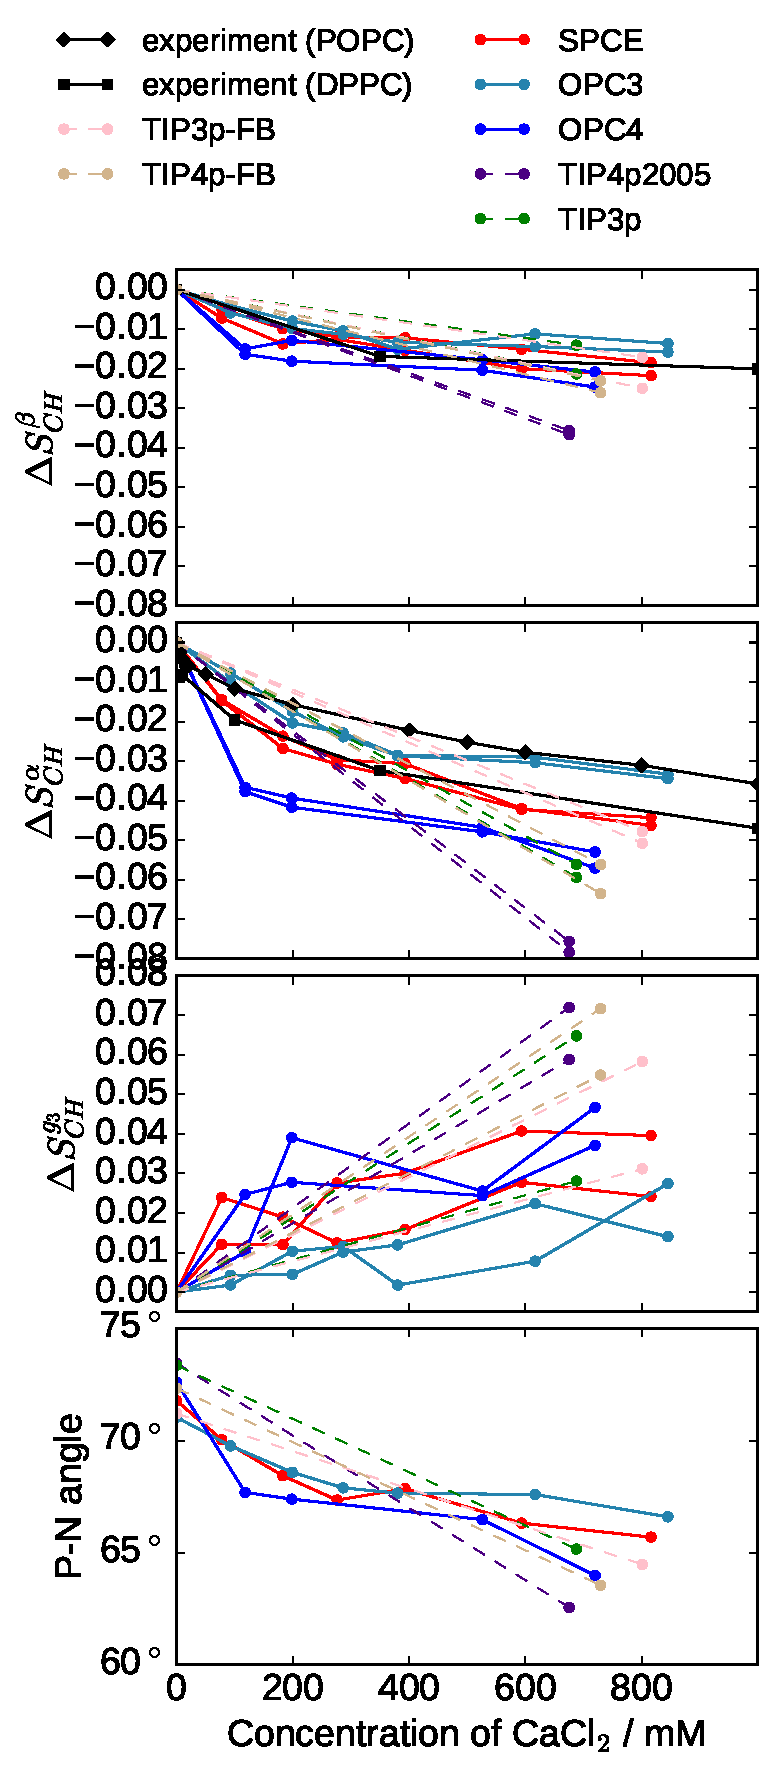
\includegraphics[width=8.0cm]{../Fig/ipython_nb/PN_angle_OrdPars-A-B-g3_L14-ECCL17_q80_sig89_CaCl_waterModels.pdf}
  \caption{\label{fig:ordPars_waterModels}
    Changes of head group order parameters of POPC bilayer as a function of CaCl$_2$ concentrations
    are shown from simulations with different force fields and water models together with experimental data 
    (DPPC \cite{akutsu81} and POPC \cite{altenbach84}). 
    Ion concentrations in bulk water are shown in x-axis. 
    Values from simulations are calculated from the of cation number density $C_{np}$
    from the region at the simulatin box edge with the constant ion concentration as [ion]=$C_{np}/0.602$.
  }
\end{figure}


\begin{figure}[tbp]
  \centering
  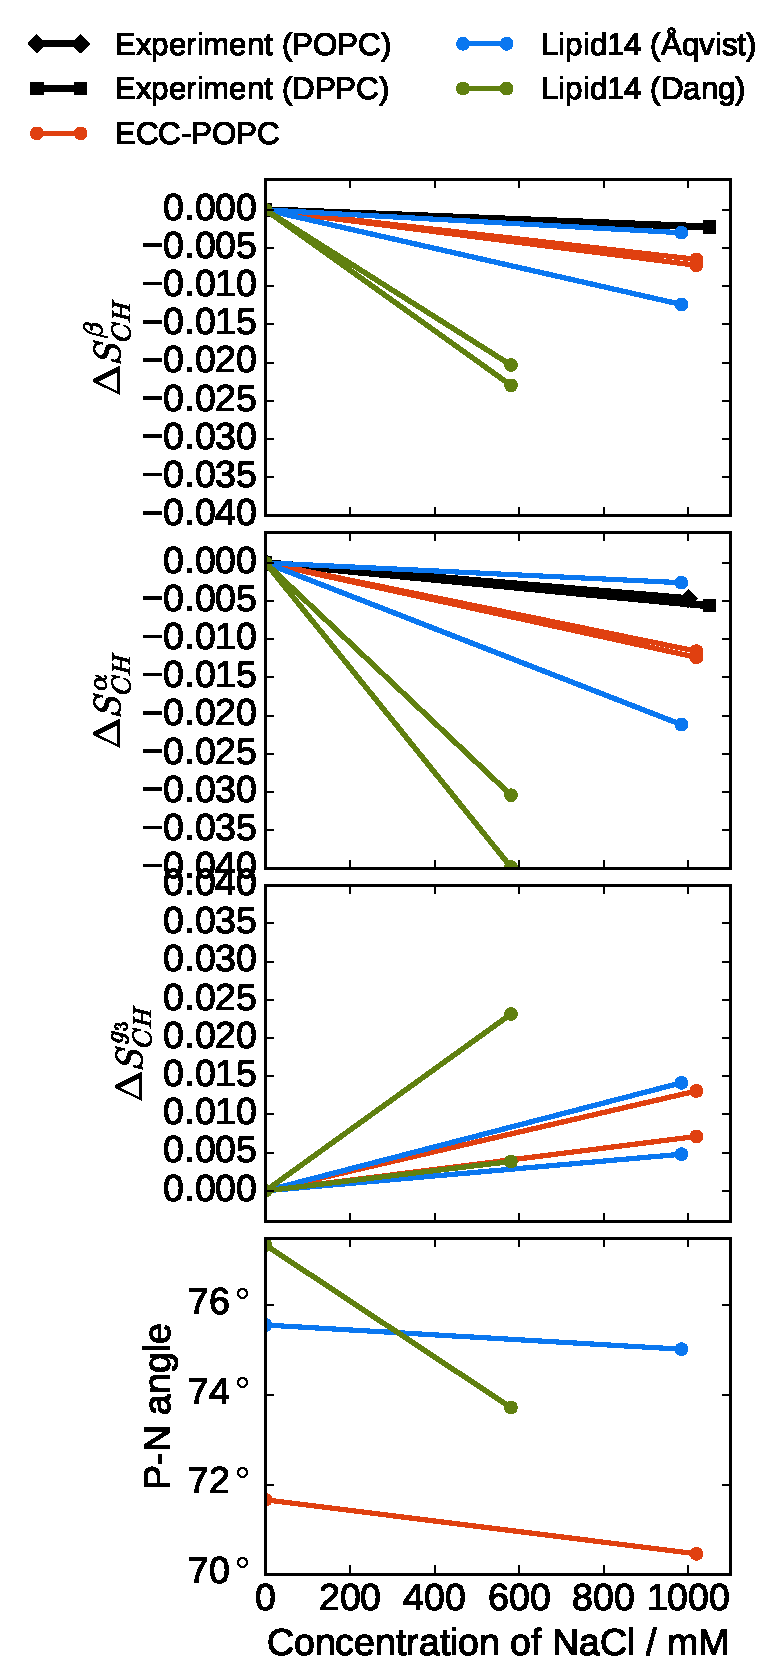
\includegraphics[width=8.0cm]{../Fig/ipython_nb/PN_angle_OrdPars-A-B-g3_L14-ECCL17_q80_sig89_NaCl.pdf}
  \caption{\label{fig:delta_ordPar_NaCl_si}
    Changes of head group order parameters of POPC bilayer as a function of NaCl concentrations
    are shown from simulations with different force fields together with experimental data \cite{akutsu81}. 
    Ion concentrations in bulk water are shown in x-axis. 
    Values from simulations are calculated from the of cation number density $C_{np}$
    from the region at the simulatin box edge with the constant ion concentration as [ion]=$C_{np}/0.602$.
    Simulation data with Lipid14 and \AA{}qvist ion parameters is taken directly from Ref. \cite{catte16}.
  }
\end{figure}


\begin{table}
  \caption{Area per lipid (APL) from different models of POPC with no ions\label{tab:apls_si} }
  \begin{tabular}{l|c c}
    model          & APL (\AA$^2$)   & Temperature [K] \\
    \hline
    Lipid14                   & 65.1$\pm$ 0.6  &  300 \\
    Lipid14 \cite{dickson14}  & 65.6$\pm$ 0.5  &  303 \\
    \hline
    ECC-lipids &        &  \\
    %Lipid14ecc0.80+sigma0.875 &        &  313    \\
    %($4.6\cdot 5.1 \, \mathrm{nm}^2$), 72 lipids patch, OPC3           & 63.2   &   313      \\
    ~ OPC3           & 62.2$\pm$ 0.6   &  300       \\
    ~ OPC3           & 64.2$\pm$ 0.6   &  313       \\
    ~ SPC/E          & 65.1$\pm$ 0.6   &  313       \\
    ~ OPC            & 64.4$\pm$ 0.6   &  313       \\
    ~ TIP4p/2005     & 66.8$\pm$ 0.6   &  313       \\
    %($9.2\cdot 10.2 \, \mathrm{nm}^2$), 288 lipids patch           & 65.5   &  313       \\ %% not done for this model with f_sigma=0.89
    %oMM small patch           & 63.65  &         \\
    %oMM 4xbig patch           & 63.7   &         \\
    \hline
    experiment   & 62.7  &  293    \\
    experiment \cite{jambeck12}\todoii{REF}{put original references, not Slipids param. paper.} & 64.3  &  303    \\
    experiment  & 67.3  &  323    \\
    experiment  & 68.1  &  333    \\
    %experiment POPE  & 56.6 &  303    \\
    \hline
  \end{tabular} \\
  \todo{Result with normal TIP3P missing?}
\end{table}


\begin{table}[btp]
  \caption{Simulation parameters}
  \label{tbl:mdpar}
  \begin{tabular}{ll}
    simulation property & parameter   \\
    \hline
    time-step           & 2~fs         \\
    equilibration time  & 100~ns  \\
    simulation time     & 200~ns  \\
    temperature         & 313~K       \\
    thermostat          & v-rescale  \cite{bussi07}   \\
    barostat            & Parrinello-Rahman, semi-isotropic \cite{parrinello81} \\
    long-range electrostatics & PME  \cite{darden93}  \\
    cut-off scheme      & Verlet \cite{Pall13}      \\
    Coulomb and VdW cut-off & 1.0~nm \\
    constraints         & LINCS, only hydrogen atoms \cite{hess97} \\
    constraints for water & SETTLE  \cite{miyamoto92} \\
    \hline
  \end{tabular}
\end{table}



% Create the reference section using BibTe
\bibliography{refs.bib}

%\newpage
%\section{APPENDIX: The NMR results reported by Tiago Ferreira}

\listoftodos

\end{document}
%
% ****** End of file aiptemplate.tex ******
